\documentclass[10pt]{article}
\usepackage{amsmath}
\usepackage{import}
\usepackage{graphicx}
\usepackage{epstopdf}
\usepackage{subfigure}
\usepackage{amsmath}
\usepackage{amssymb}
\usepackage{url}
\usepackage{units}
\usepackage{hyperref}
\usepackage{tabularx}
\usepackage{cancel}
\usepackage{longtable}
\usepackage{breqn}
\usepackage{mathtools}
\usepackage{graphics}
\usepackage{tabularx}
\usepackage{color}
\usepackage{indentfirst}
\usepackage[utf8]{inputenc}
\usepackage[margin=1in]{geometry}
\title{Analysis Proposal}
\author{Benedikt Riedel}
\date{\today}

\begin{document}

\maketitle

\section{Detector Stability}

Analysis of the detector stability using of partial detectors, 40-string though 79-string configuration, in \cite{vbaumaster} and \cite{mkrasbergtalk} showed that there was significant noise due to the freeze-in process. For the full detector, the same effect is seen, see Figure~\ref{fig:snscalerIC86ItoIII} and Figure~\ref{fig:snscalerIC86I}. As the freeze-in process subsides, the annular modulation of the muon rate with temperature, see Figure~\ref{fig:muonseasonal}, causes the detector rate to have a sinusoid-like time dependence. This becomes the most significant contribution to detector instability over time. A similar effect can also be seen in the detector SLC rate, see Figure~\ref{fig:SLCrateIC86ItoIII}. 

\begin{figure}[h]
  \begin{center}
    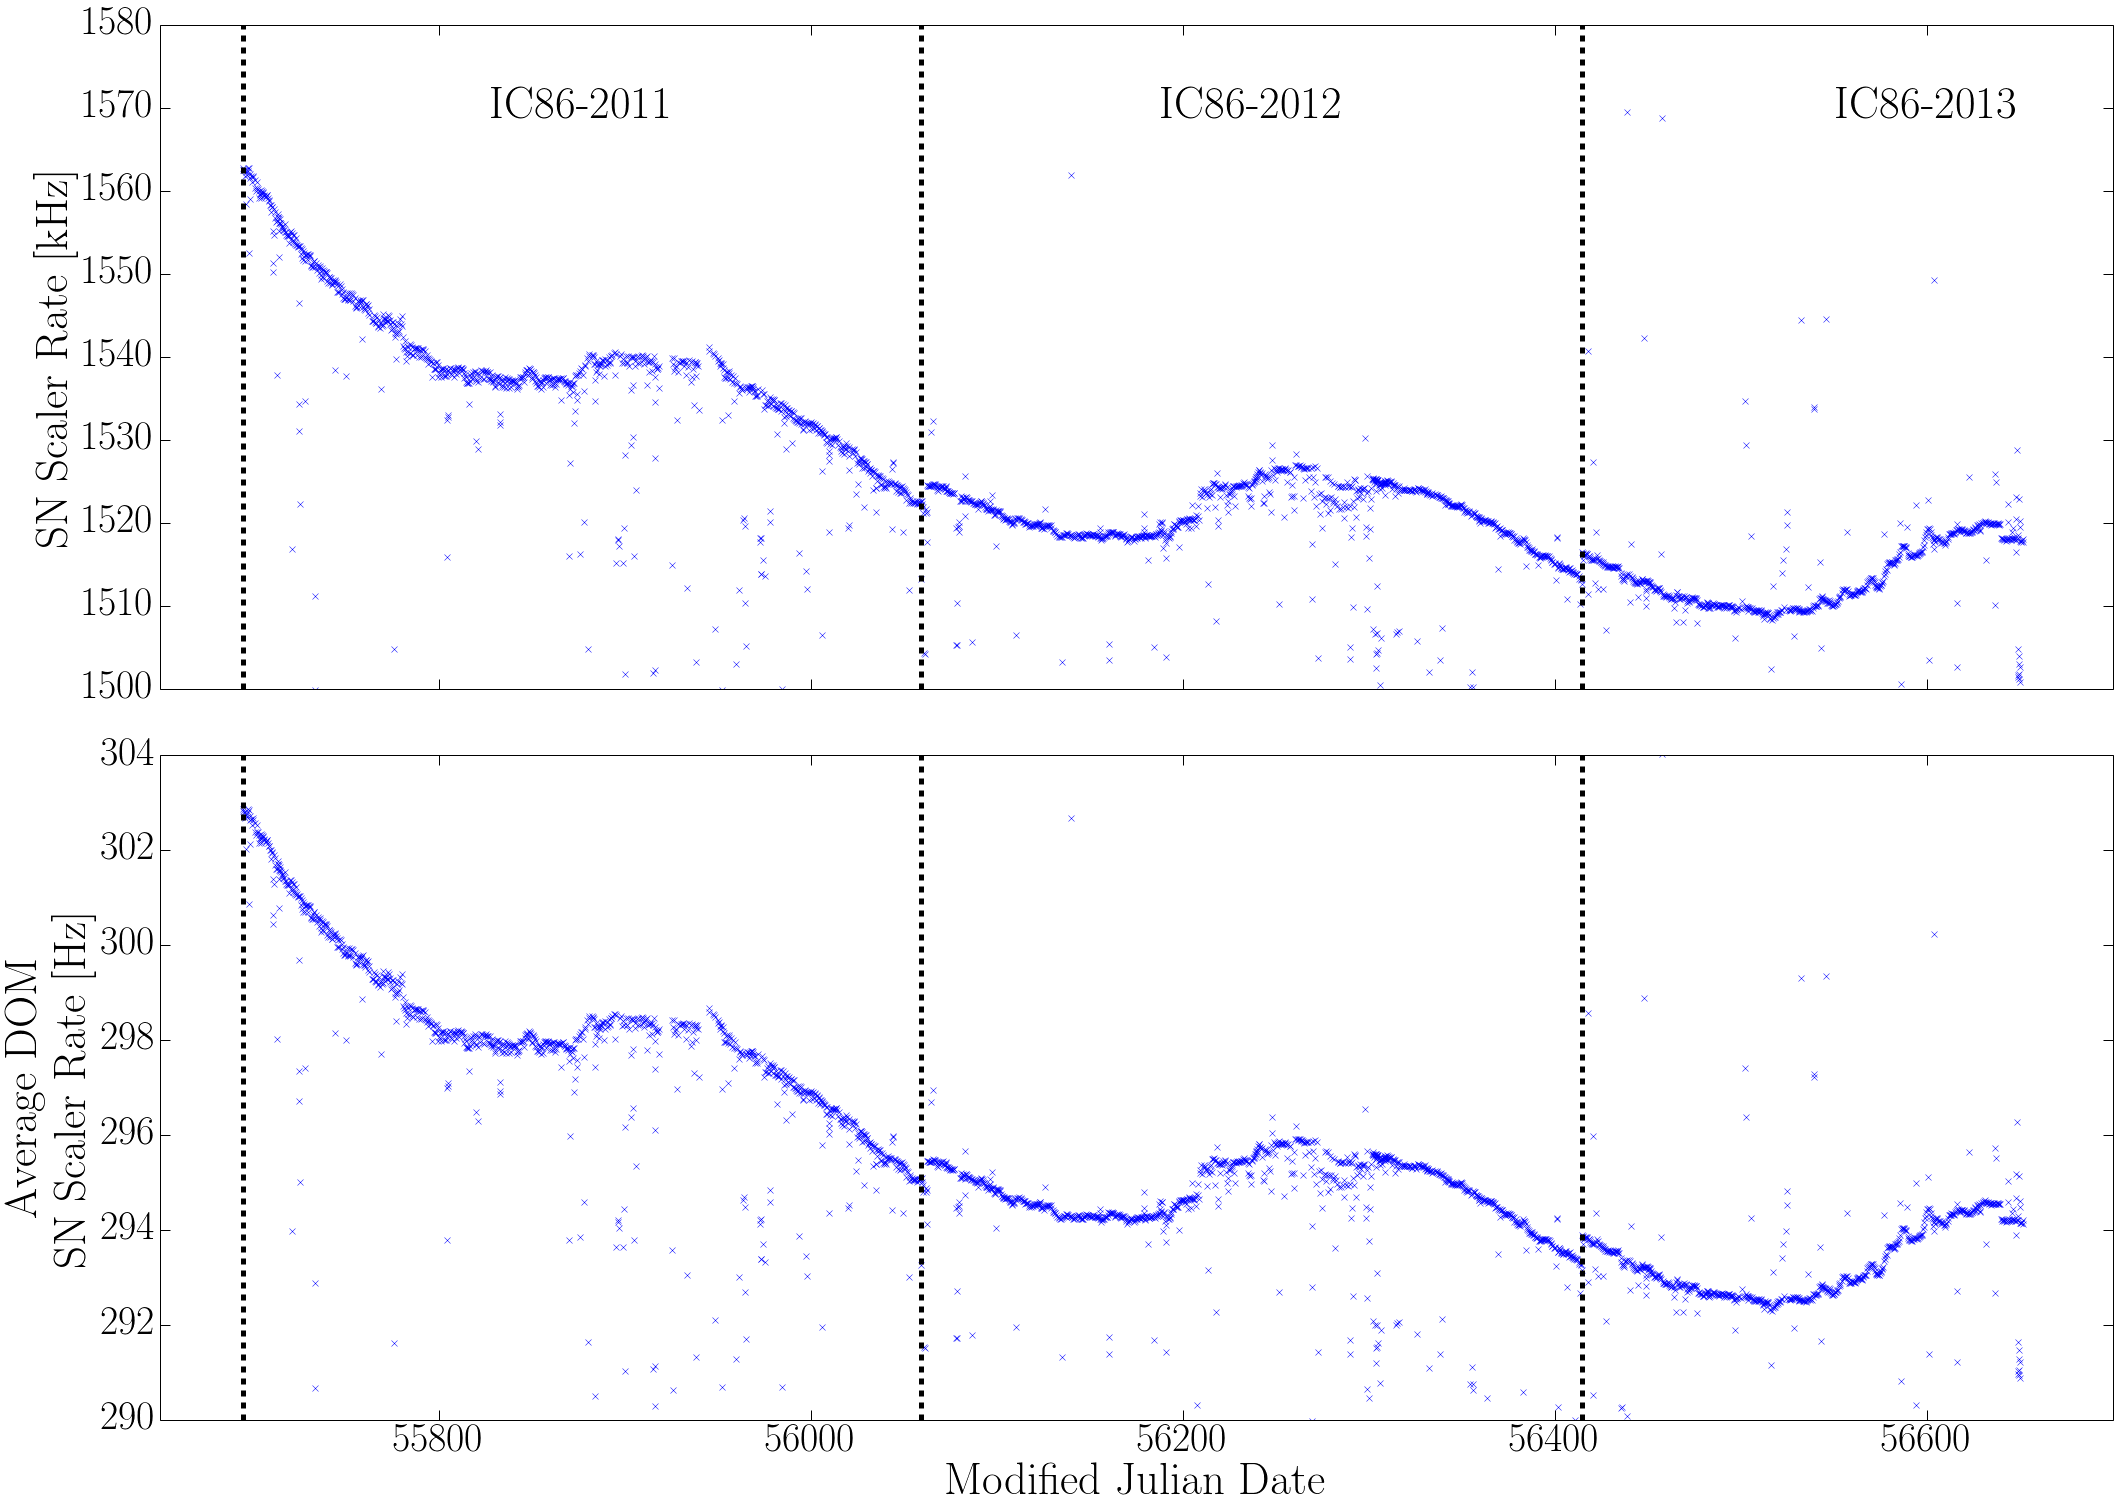
\includegraphics[width=1\textwidth]{./figures/SNScalerRateTotalAvgIC86I_III.png} 
  \end{center}
  \caption{ Total (Top) and Average (Bottom) Supernova Scaler Rate as function of time. The seasonal variation of the muon rate can be seen as a sinusoid-like pattern in the data, while the affect of the freeze-in can be seen clearly in the rate decay in IC86-2011. There is also a continual decay in rate of unknown origin.\\
  Note: Top plot is in Kilohertz, while bottom plot is in Hertz.\label{fig:snscalerIC86ItoIII}}   
\end{figure}

\begin{figure}[h]
  \begin{center}
    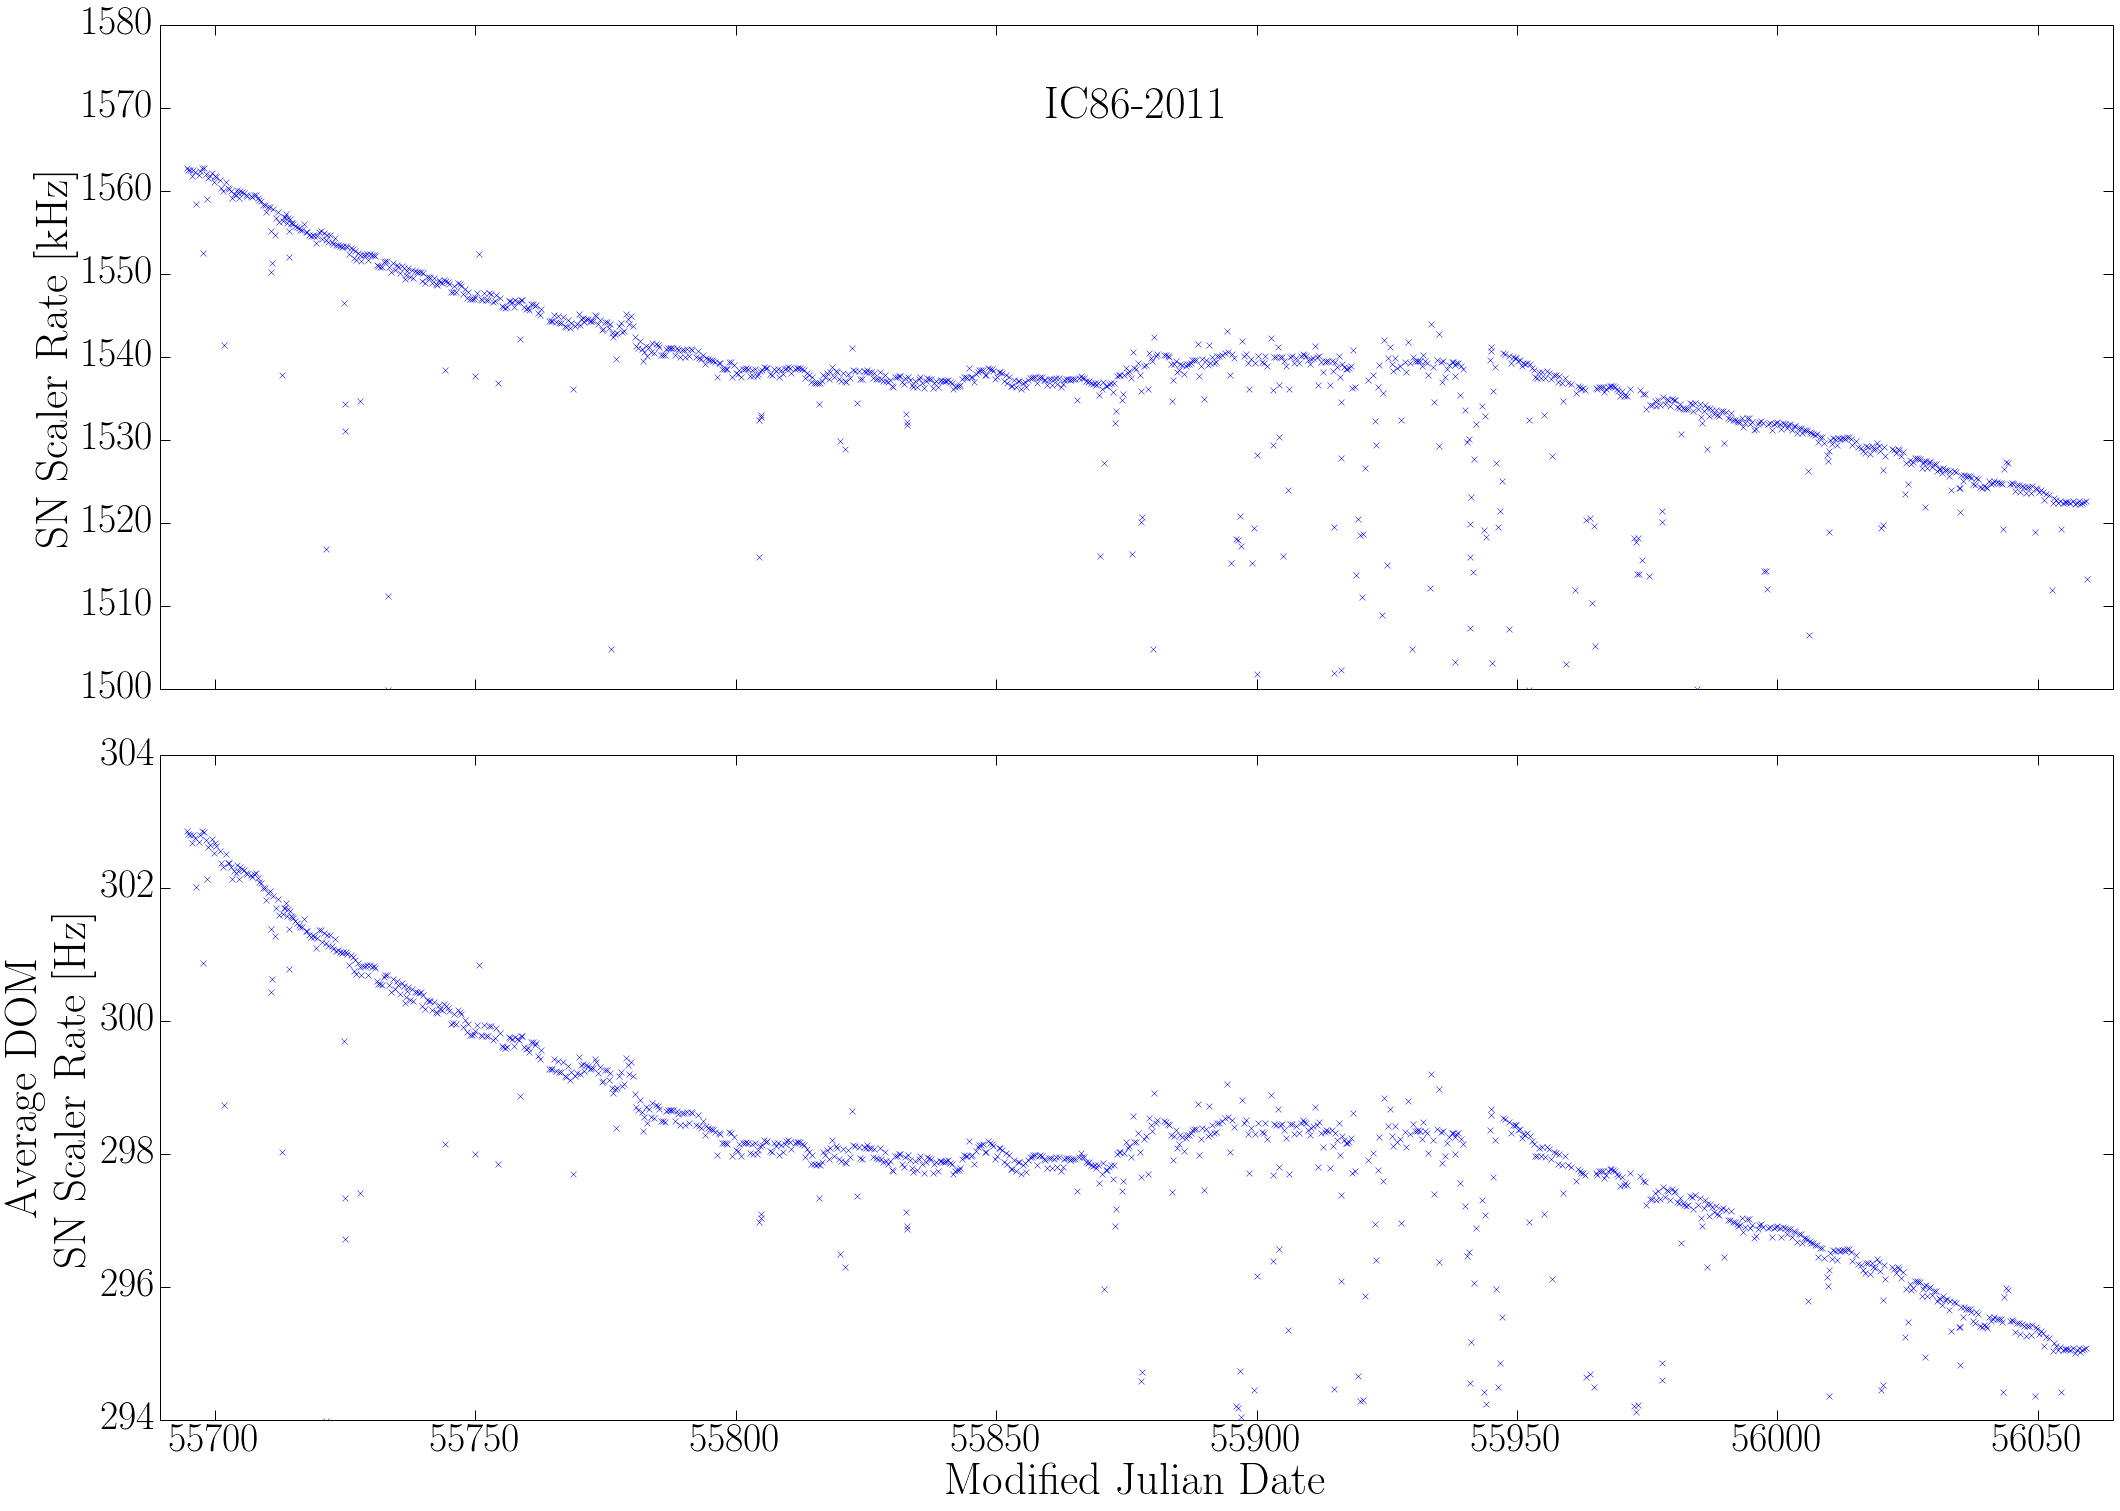
\includegraphics[width=1\textwidth]{./figures/SNScalerRateTotalAvgIC86I.png} 
  \end{center}
  \caption{ Total (Top) and Average (Bottom) Supernova Scaler Rate as function of time for the first year of IC86, IC86-2011. The freeze-in process dominates the rate over the course of the first half of IC86-2011, but becomes subdominant due to effects from muons. \\
  Note: Top plot is in Kilohertz, while bottom plot is in Hertz.\label{fig:snscalerIC86I}}   
\end{figure}

\begin{figure}
  \begin{center}
    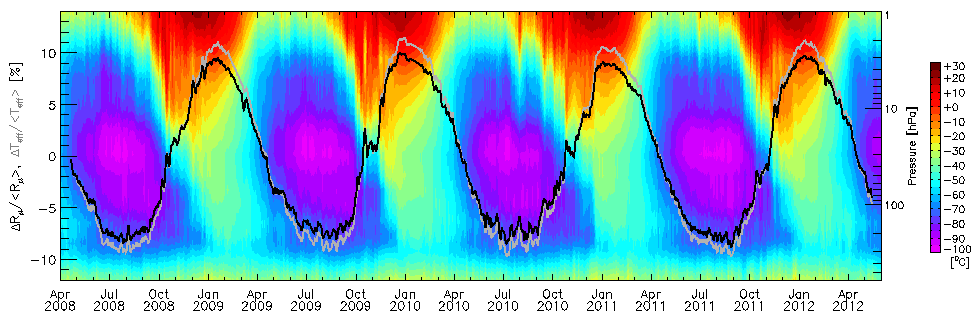
\includegraphics[width=1\textwidth]{./figures/airs_dst_teff_daily.png}
  \end{center}
  \caption{Black line shows muon rate seasonal modulation as percentage deviation from average. For reference, the atmospheric temperature as a percentage deviation from average in grey and atmospheric pressure. \label{fig:muonseasonal}}   
\end{figure}

\begin{figure}
  \begin{center}
    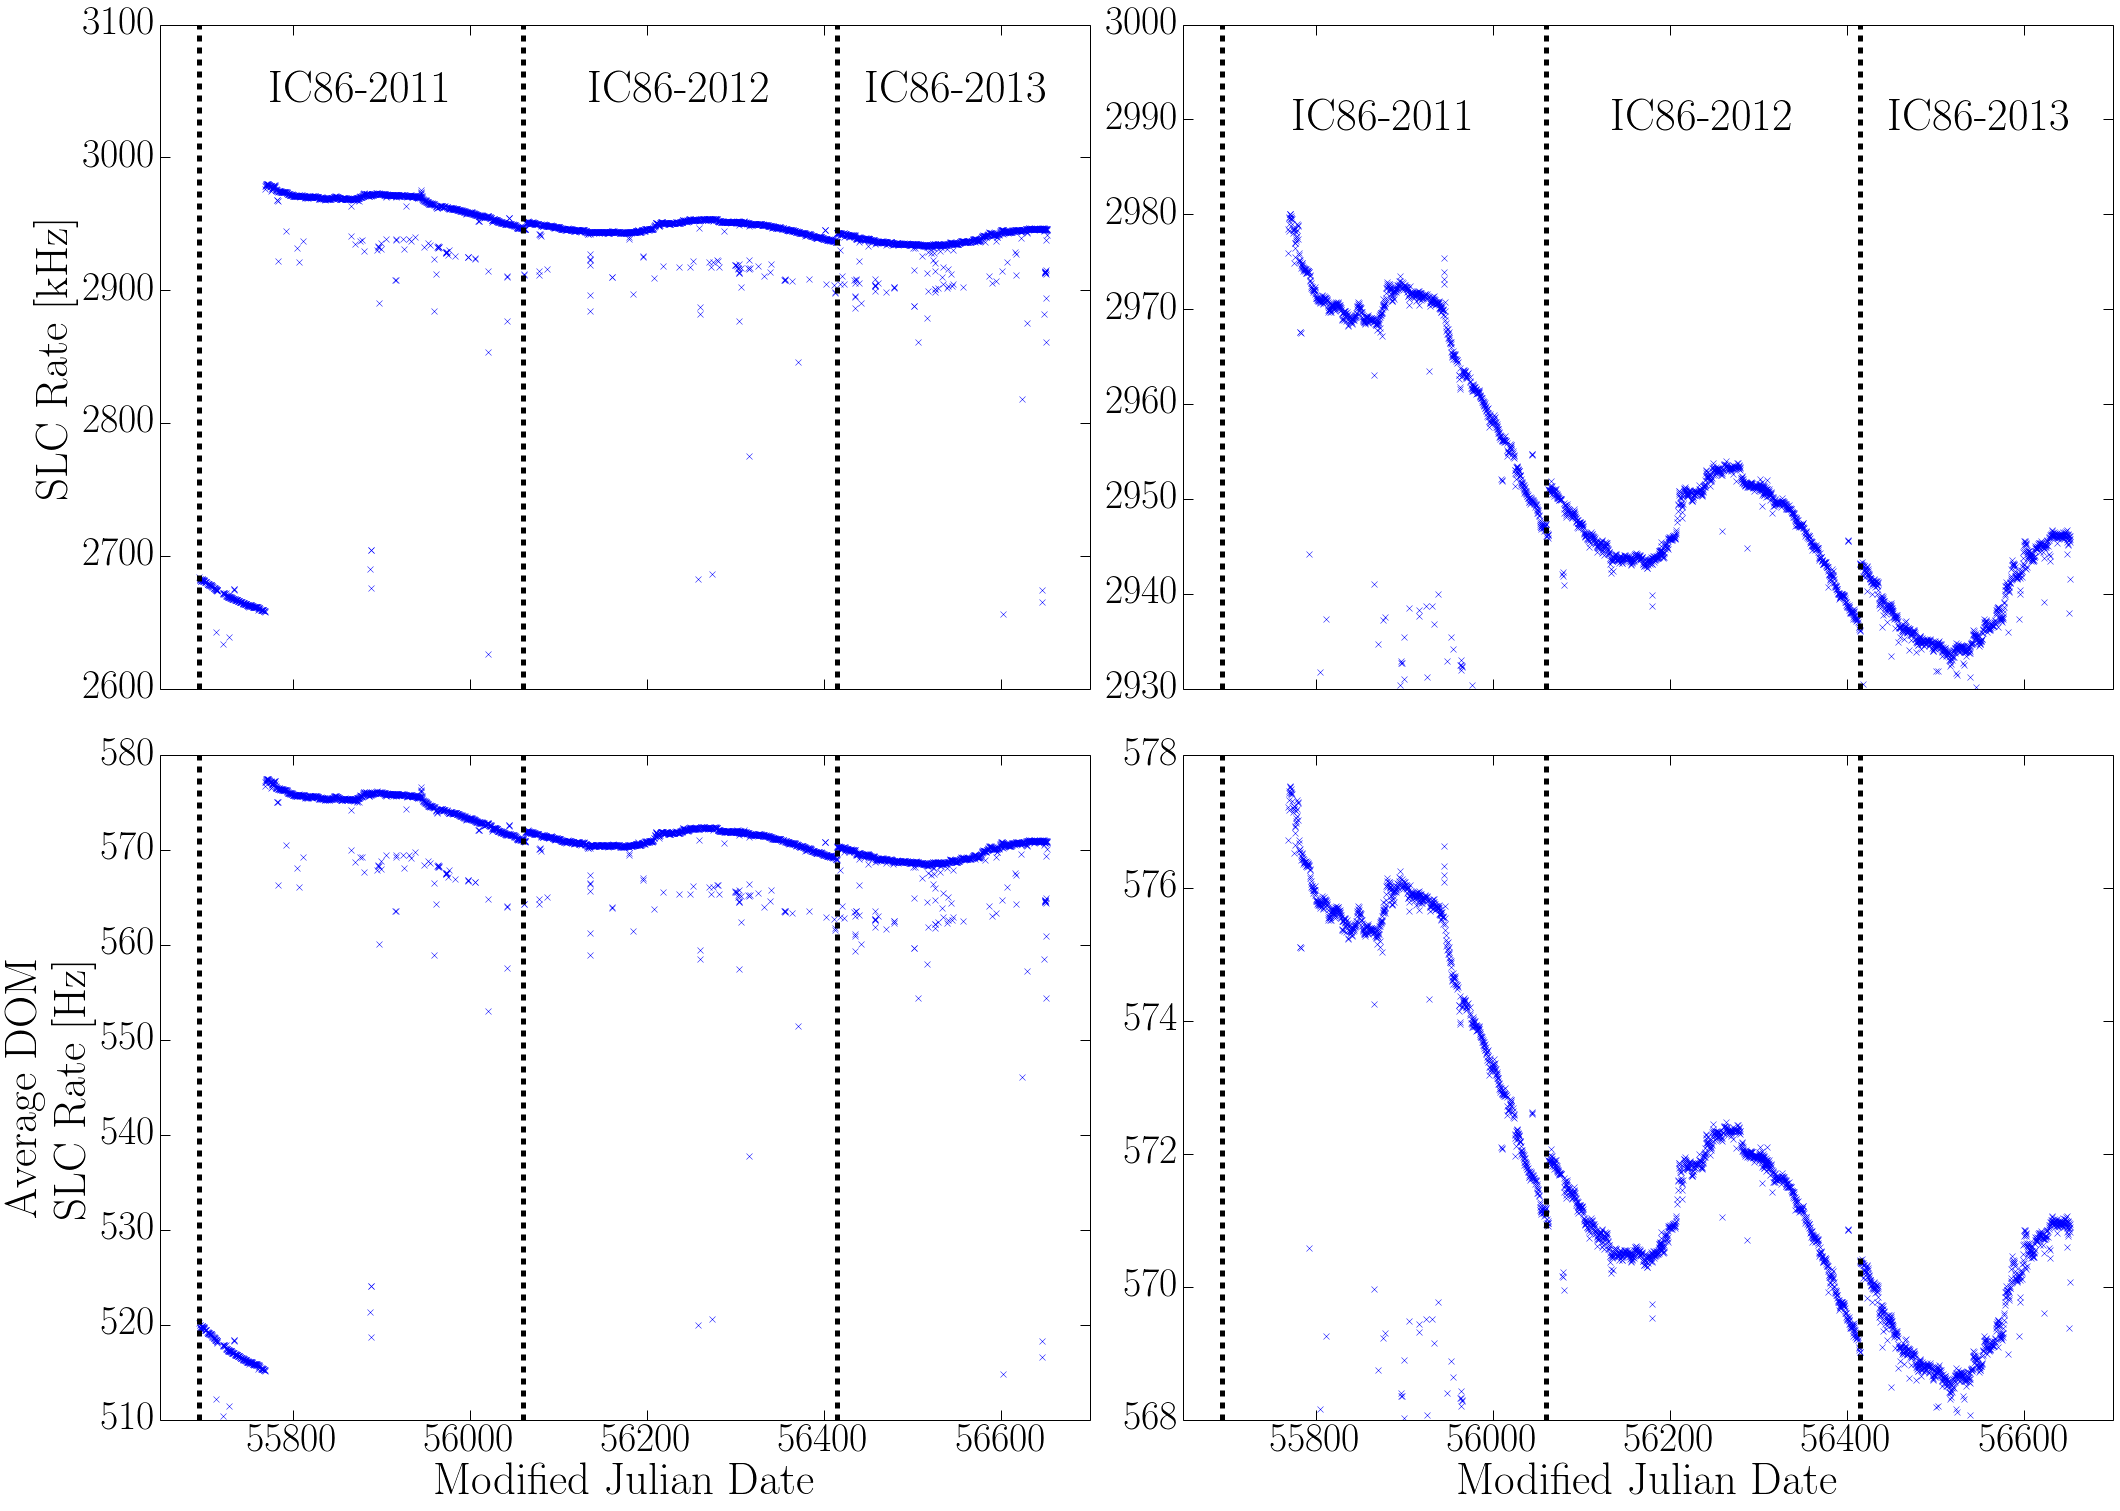
\includegraphics[width=1\textwidth]{./figures/AvgSLCRateIC86I_III.png} 
  \end{center}
  \caption{ Total (Top Panels) and Average (Bottom Panels) SLC as function of time. The seasonal variation of the muon rate can be seen as a sinusoid-like pattern in the data, while the affect of the freeze-in can be seen in the decay in the rate over the course IC86-2011 to -2013. The jump in rate about a quarter into IC86-2011 is due to changes in the deadtime by a factor of 10 (0.25\% to 0.025\%) and the subsequent addition of non-Poissonic noise to the SLC rate.\\
  Note: Top plots are in Kilohertz, while bottom plots are in Hertz.\label{fig:SLCrateIC86ItoIII}}   
\end{figure}

\begin{figure}[h]
  \begin{center}
    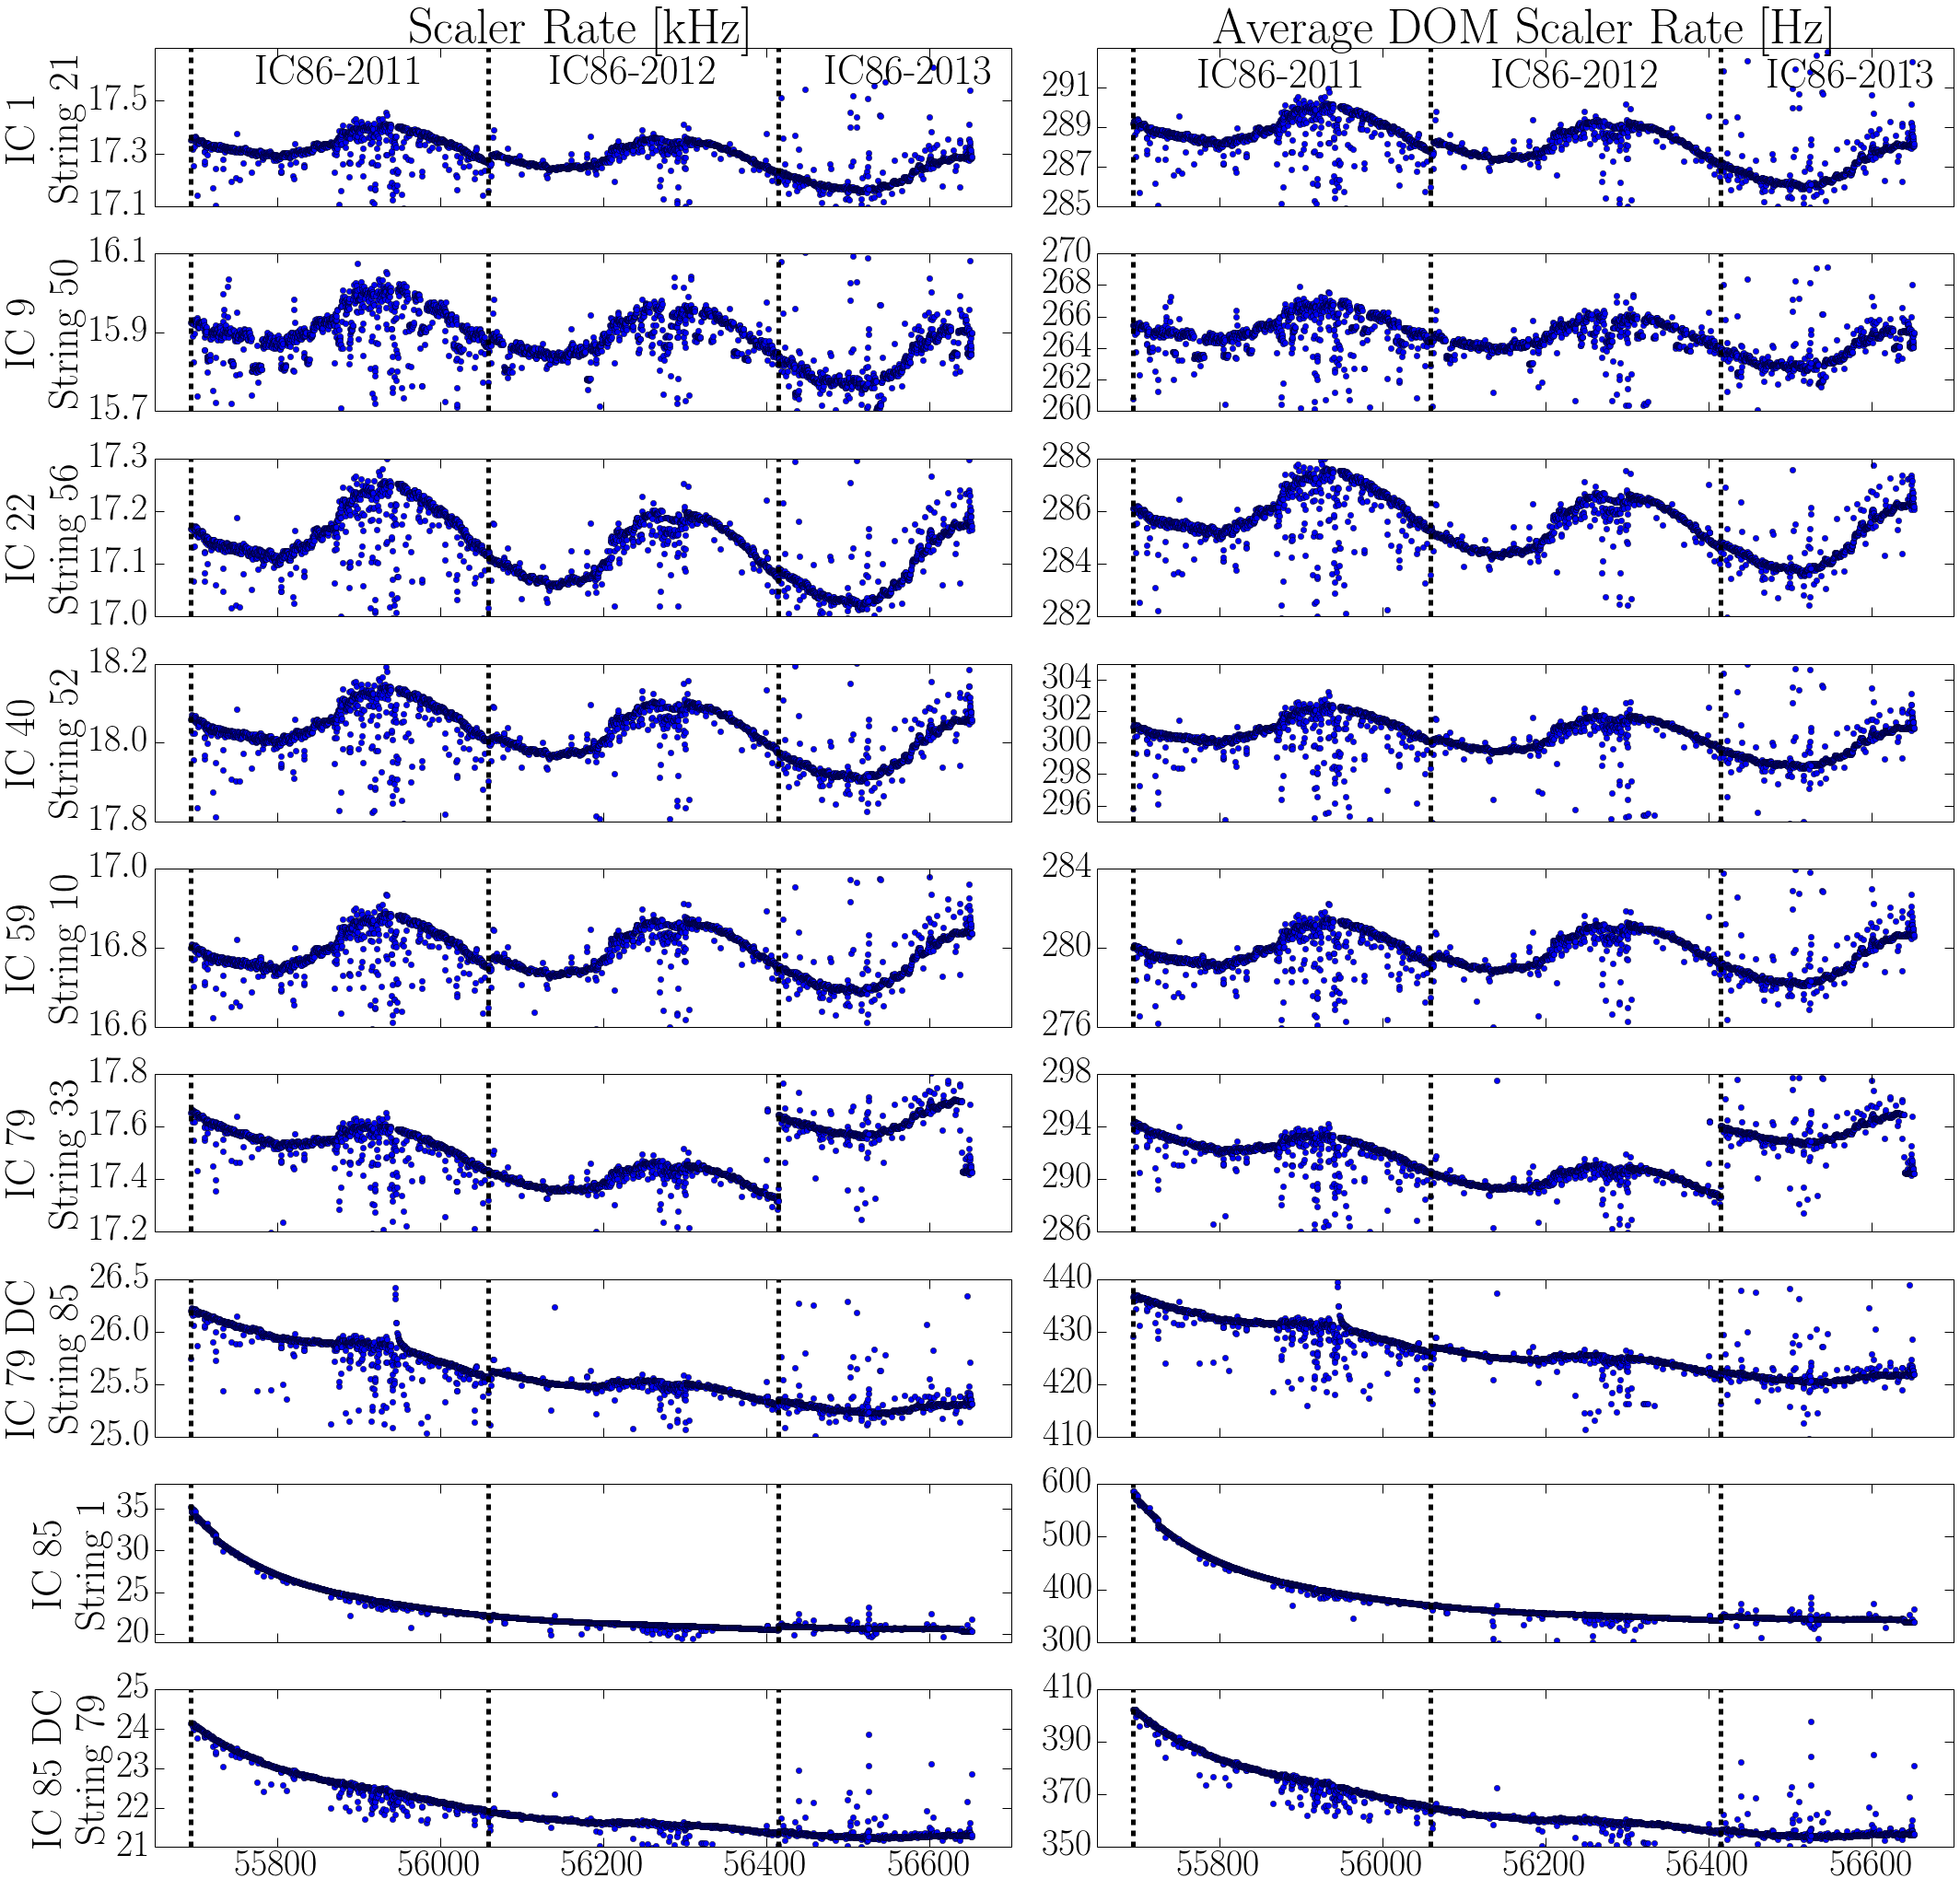
\includegraphics[width=1\textwidth]{./figures/SNScalerRateAgeIC86I_III.png}
  \end{center}
  \caption{Supernova Scaler Rate of Strings that have been deployed at different generations of the detector. String 21 for IC1, String 50 for IC9, String 56 for IC22, String 52 for IC40, String 10 for IC59, String 33 for IC79, String 85 for IC79 DeepCore, String 1 for IC86, String 79 for IC85 DeepCore. \label{fig:scalerrateage}}   
\end{figure}

Figure~\ref{fig:snscalerIC86ItoIII} and~\ref{fig:SLCrateIC86ItoIII} also reveal a continual decay in the detector rate throughout the operation of the full detector configuration. Comparison of supernova scaler rate for the 86-string configuration for strings deployed at all the different construction cycles, see Figure~\ref{fig:scalerrateage}, shows that the decay is on-going even several years after deployment. Similarly, the freeze-in progresses has a depth dependence the, see Figure~\ref{fig:scalerratedepth}. The origin of this decay is unknown. There are multiple possible explanations that can be examined from the data:


\begin{figure}[h]
  \begin{center}
    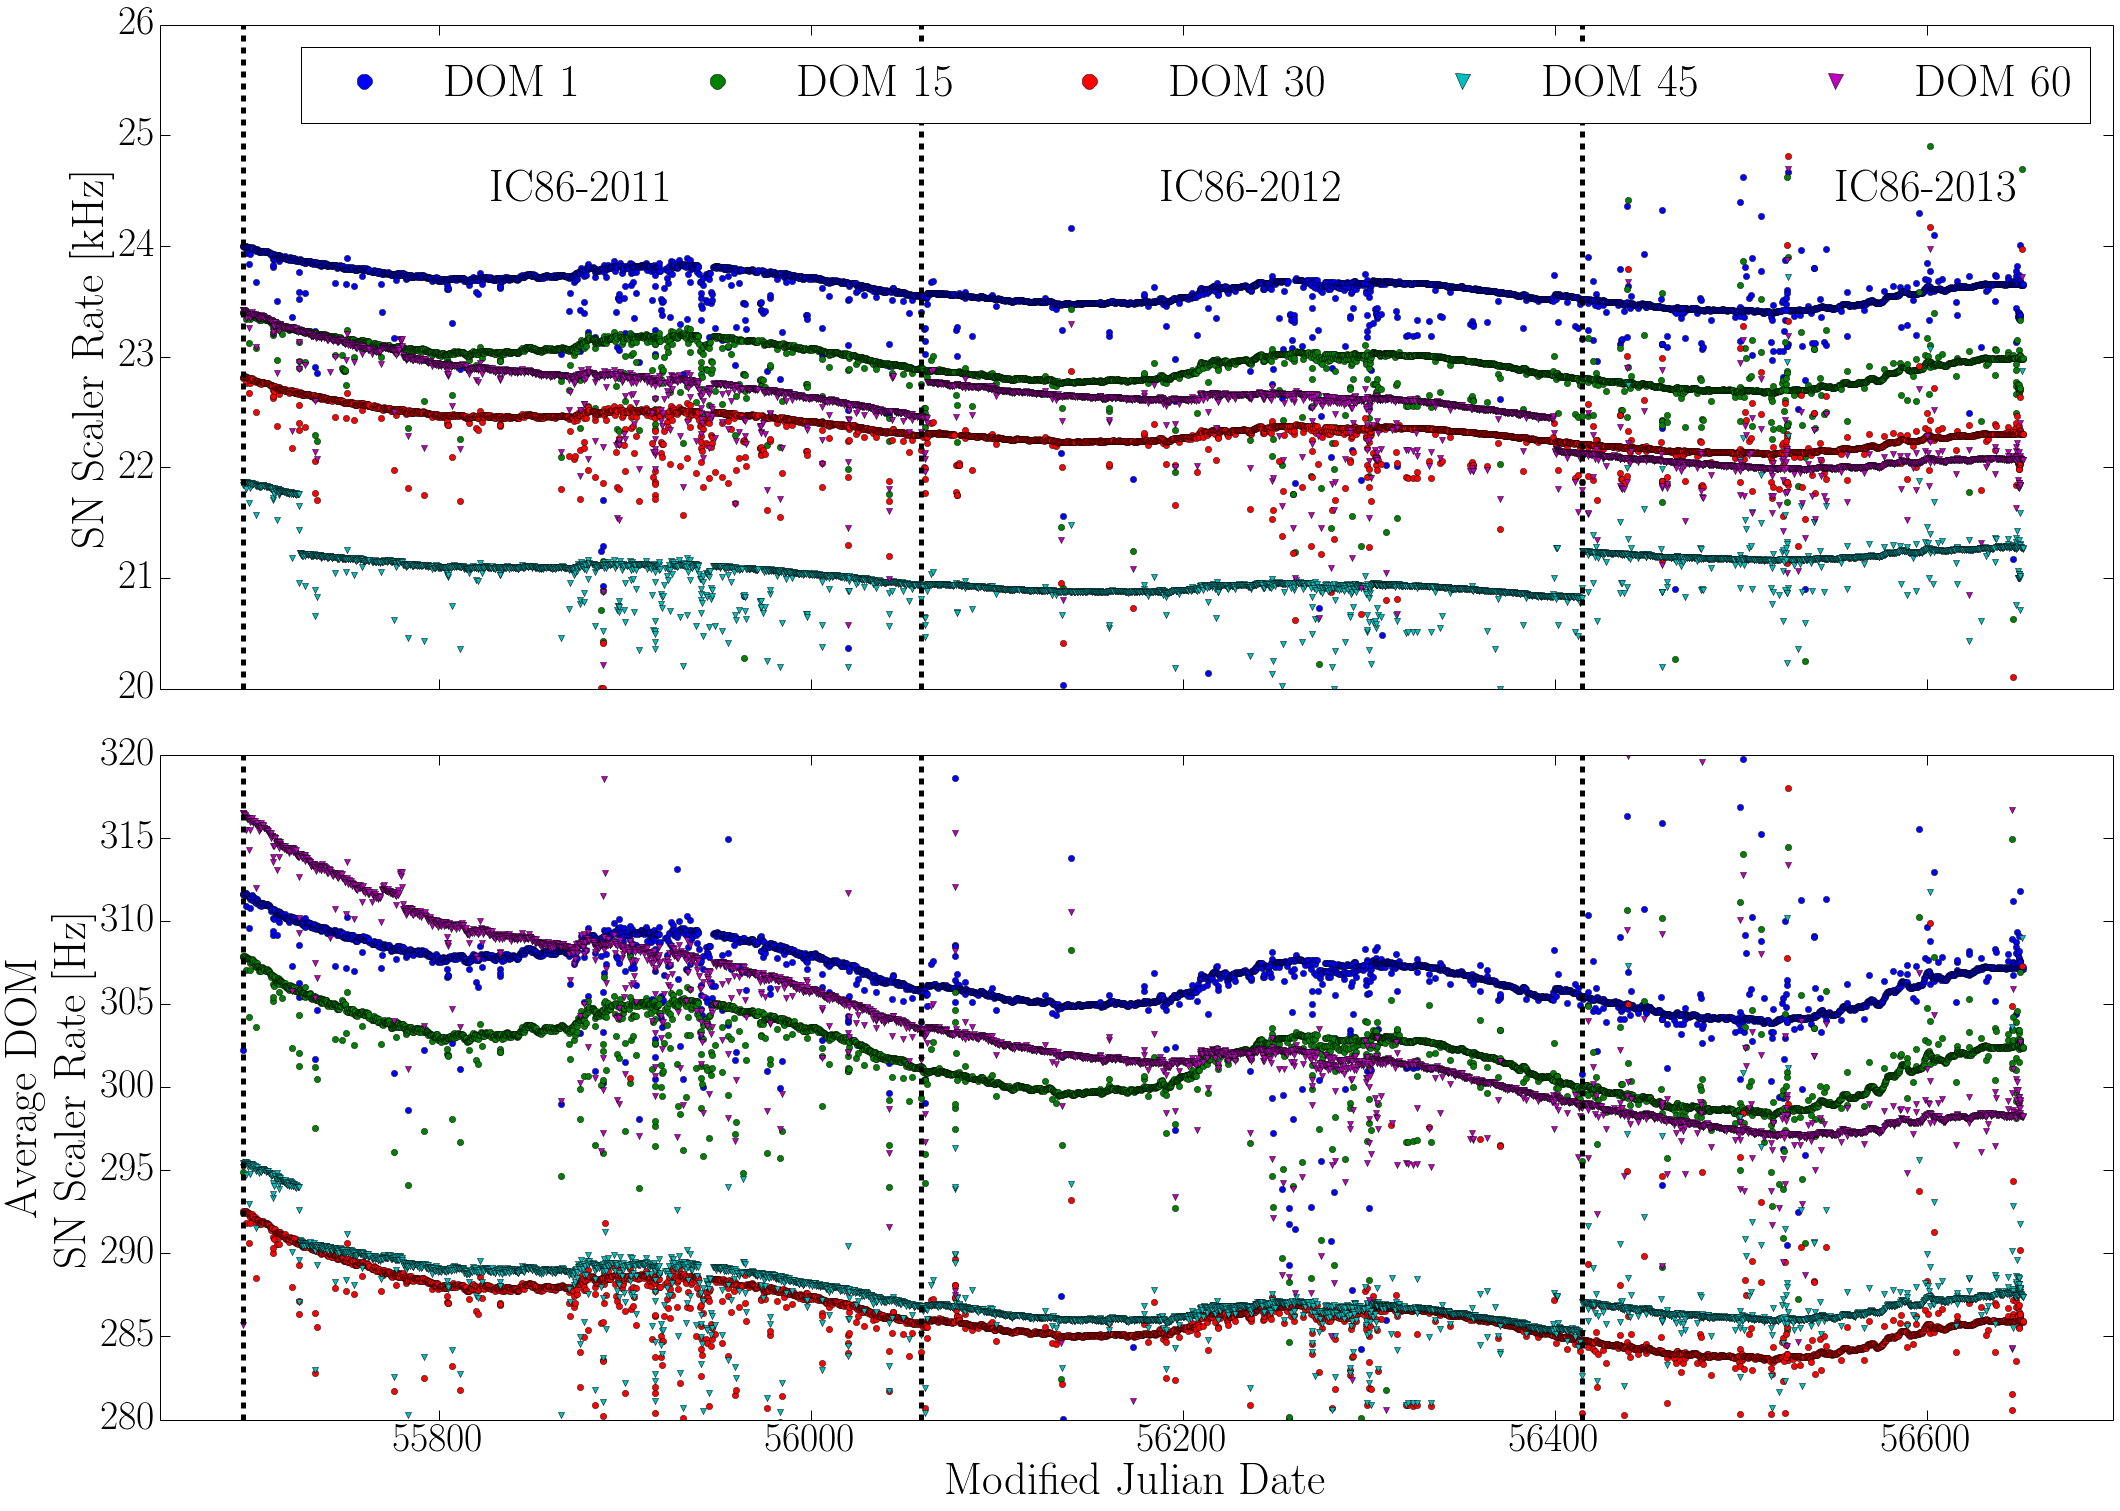
\includegraphics[width=1\textwidth]{./figures/SNScalerRateLayersIC86I_III.png}
  \end{center}
  \caption{Supernova Scaler Rate of DOMs at different depths. DOM 1 are DOMs at the top of the detector, DOM 15 are in the middle of the top half, DOM 30 are in middle and inside the dust layer, DOM 45 are in the middle of the bottom half of the detector, and DOM 60 are the bottom of the detector. This excludes the DOMs from DeepCore as their geometry is different. \label{fig:scalerratedepth}}   
\end{figure}

\begin{itemize}
  \item Construction effects: Continuation of the freeze-in process
  \item Detector effects: Detector aging and drift of detector settings away from optimal values
\end{itemize}

The freeze-in process continues even after the ice appears to be solid, as shown by the ``Swedish Camera'', a camera system deployed in the deep ice at the end of String 80. Recordings from the ``Swedish Camera'' have shown that the ice surrounding the bore hole continues to change over the years. The air and particles trapped in the ice from drilling and refilling the bore holes are being pressed into a central column. This processes appears to be on-going and may cause low levels of triboluminescence similar to those associated with the solidification process that are seen as a decay in the supernova scaler, see Figure~\ref{fig:snscalerIC86I}. 

To establish the decay rate for the individual DOMs, a fit of:

\begin{equation}
  R(t) = A + R_{\mu} (t) + \left( C \textrm{exp}\left( -\tau t \right) \right)
  \label{eq:scalerratebreakdown}
\end{equation} 

\noindent where $A$ is baseline noise from the DOM, $R_{\mu}$ is the time-dependent atmospheric muon rate contribution to the scaler rate, and $C \textrm{exp}\left( -\tau t \right)$ is the contribution of the decay rate to the SN scaler rate, has to be performed on the SN scaler rate. \cite{vbaumaster} used the IceCube trigger-level data to estimate the atmospheric muon contribution. This data however has a significantly higher energy threshold, $\approx \unit[400-800]{GeV}$ depending on depth versus $\approx \unit[1]{TeV}$ and lower rate than the scaler data, i.e. $\approx \unit[2100]{Hz}$ versus $\approx \unit[5200]{Hz}$. 

\begin{figure}[h]
  \begin{center}
    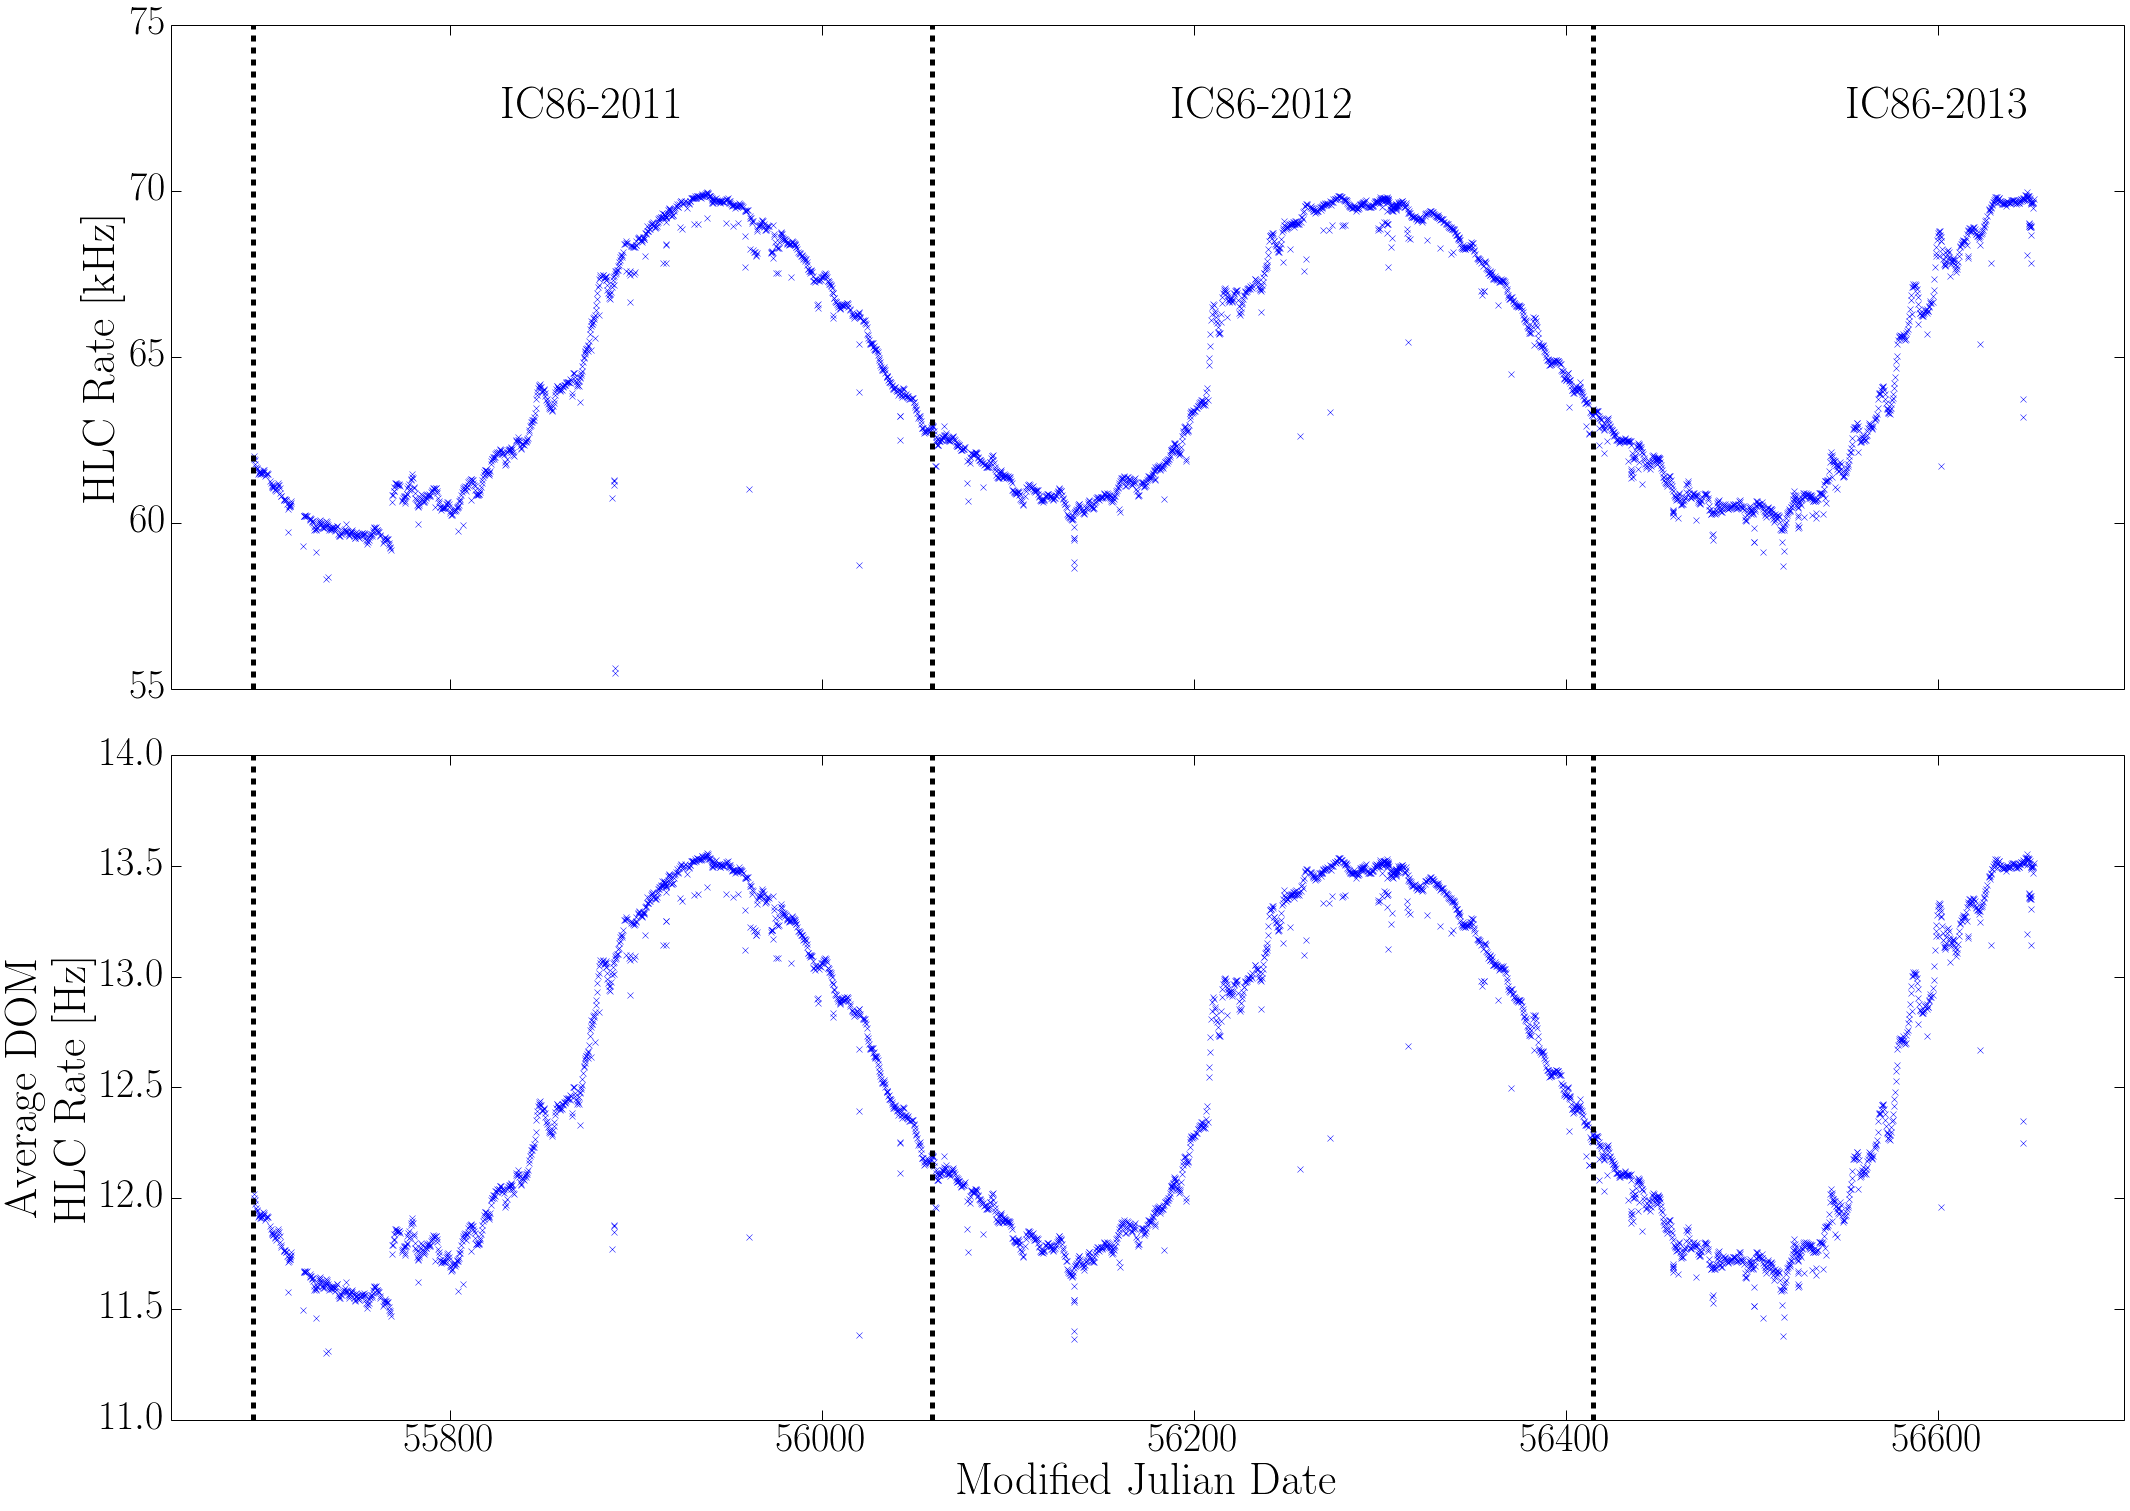
\includegraphics[width=1\textwidth]{./figures/AvgHLCRateIC86I_III.png}
  \end{center}
  \caption{Total (Top) and Average (Bottom) HLC as function of time.\label{fig:HLCratevstimenocorrection}}}   
\end{figure}

The HLC rate for individual DOMs from the pDAQ log-files provides an estimate of the atmospheric muon effect with a lower energy threshold. This HLC rate mimics the effect of the atmospheric muons, see Figure~\ref{fig:HLCratevstimenocorrection}. A correction factor, $R_{C}$, has to be subtracted from the HLC rate, as there are HLC due to noise. Assuming that the SLC rate is purely Poissonic, $R_{C}$ can be esimated using

\begin{equation}
  R_{C} = 2 \Delta t R_{3}\left( R_{1} + R_{2} + R_{4} + R_{5} \right)
\end{equation}

\noindent where $R_{3}$ is the rate of the central DOM, and $R_{1, 2, 4, 5}$ is the rate of the surrounding DOMs. The rate for each DOM is estimated using the SLC rate for each DOM. The remaining rate can be attributed to the effect of atmospheric muons, see Figure~\ref{fig:fig:HLCratevstimecorrected}.

\begin{figure}[h]
  \begin{center}
    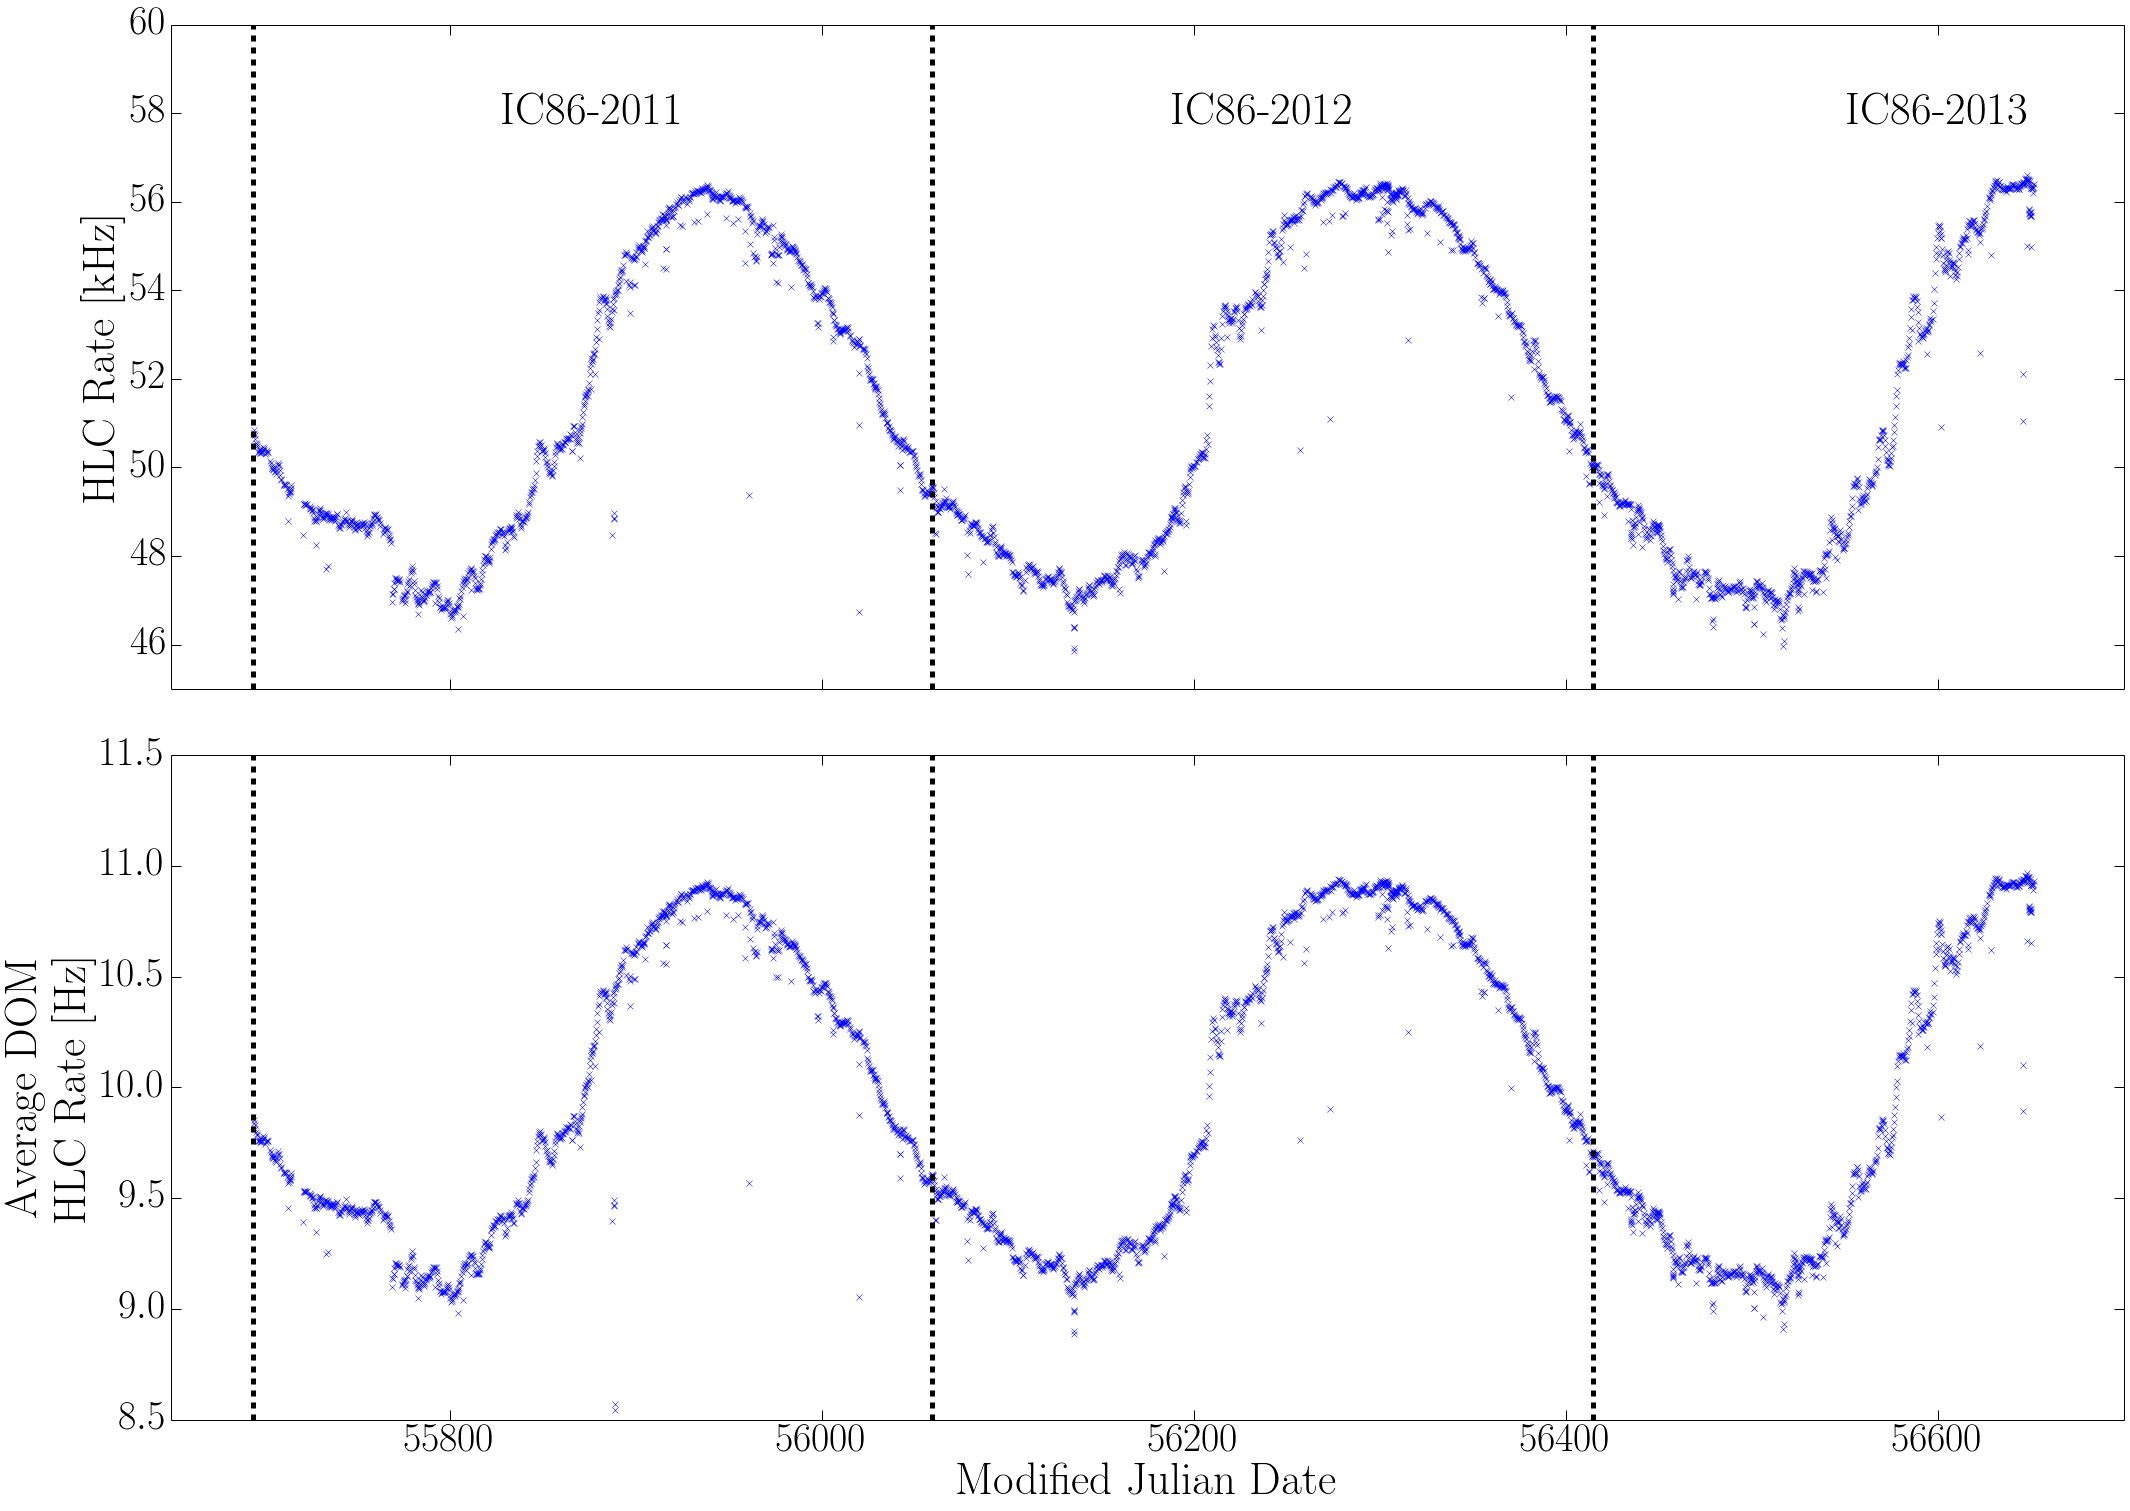
\includegraphics[width=1\textwidth]{./figures/AvgHLCRateIC86I_III_Minus_Coincidence.png}
  \end{center}
  \caption{Total (Top) and Average (Bottom) HLC as function of time after coincidence rate is removed. \label{fig:HLCratevstimecorrected}}}   
\end{figure}

The response to atmospheric muons is different for SN scaler rate and the HLC rate. SN scalers have a much longer deadtime compared to SLC and HLC rates, \unit[250]{$\mu$s} versus $\approx$\unit[2.5]{$\mu$s}. The HLC rate requires two DOMs to participate, while SN scalers is sensitive to individual DOMs. This is pre-dominately a concern for DOMs on the edge of the detector. The definition of $A$ and $R_{\mu} (t)$ from Equation~\ref{eq:scalerratebreakdown} has to therefore be changed slightly to estimate the atmopsheric muon contribution to the SN scaler rate. $A$ aborbs the average atmoshperic muon rate that effect the SN scalers, while $R_{\mu} (t)$ becomes the deviation of the atmopsheric muon rate from this average. Equation~\ref{eq:scalerratebreakdown} is more apbtly described by

\begin{equation}
  R(t) = R_{\textrm{\DOM}} + R_{\mu} + B \Delta R_{\textrm{HLC}} (t) + \left( C \textrm{exp}\left( -\tau t \right) \right)
  \label{eq:scalerratenewbreakdown}
\end{equation}

\noindent where 

\begin{equation}
   \Delta R_{\textrm{HLC}} (t) = R_{\textrm{HLC}} (t) - \langle R_{\textrm{HLC}} \rangle
\end{equation}

\noindent and $B$ is scaling factor that compensates for the difference in HLC and SN scaler sensitivity. $B$ can be found by letting it freely float while fitting for $\tau$ in Equation~\ref{eq:scalerratenewbreakdown}. This subtraction method has already proven usable to reduce the affect of atmospheric muons ont the SLC rate, see Figure~\ref{fig:SLCratewandwoHLCmuon}. If the fitting does not work properly one can estimate the scaling factor by simulating atmohsperic muons without detector noise and determine if the scaling factor of SLC atmospheric muons rate to HLC atmospheric muons rate as a function of energy. 

\begin{figure}[h]
  \begin{center}
    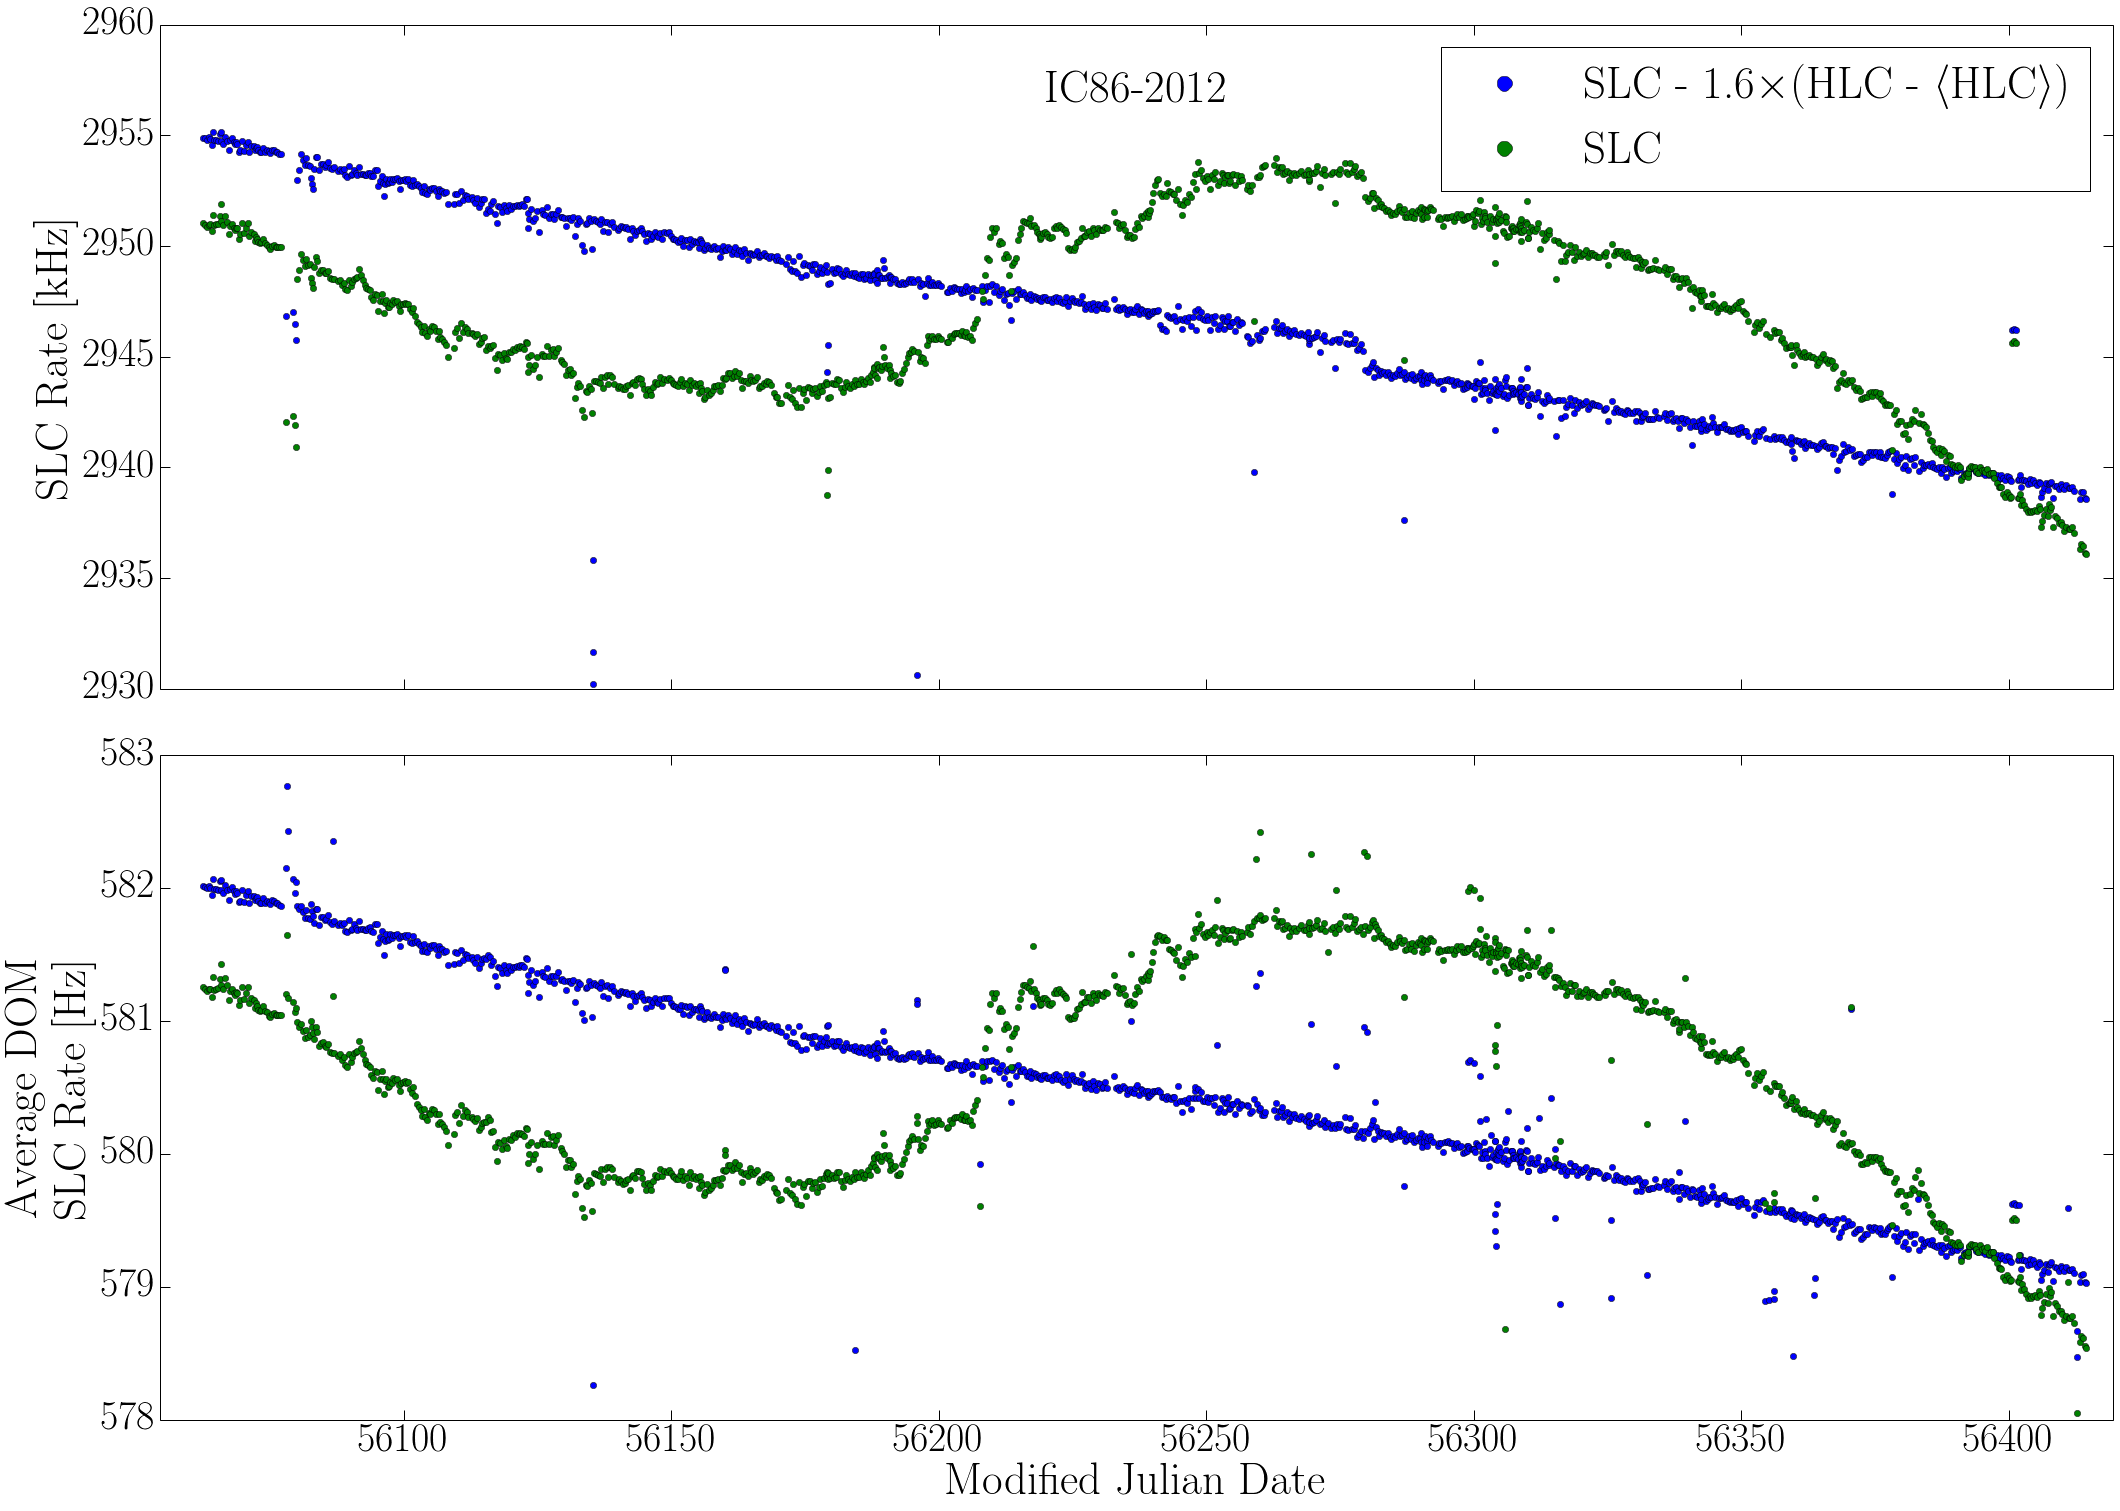
\includegraphics[width=1\textwidth]{./figures/SLCRateHLCsubtractionIC862.png}
  \end{center}
  \caption{Total (Top) and Average (Bottom) SLC as function of time for IC86-2012 with and without muon substraction \label{fig:SLCratewandwoHLCmuon}}}   
\end{figure}


 % in order to esimate The rate of individual hits attributed to atmospheric muons has to estimated from simulation. The single hit rate in data can be estimated by simulating muons with a known spectrum and determining the per-DOM single hit and HLC rate. The per-DOM single hit rate can than be scaled according to the ratio of the per-DOM HLC rate between simulation and data. 

% This fit assumes that the sinusoidal-like effect produced by the atmospheric muons averages out over time and is absorbed into the term for the average Poisson rate of DOM noise and atmospheric muons, $A$. A fit to the data from the dust layer would suppress the effect of the muon background, see Figure~\ref{fig:scalerratedepth} Panel for DOMs at position 35, but would not capture the depth dependence of the freeze-in process. 

 % In order to verify this, a comparison between the freeze-in rate established from ``Swedish Camera'' data and the decay rate seen at the bottom of the detector should be performed.

% This comparison would show whether the decay rate is associated with the freeze-in process surrounding the bore hole and its possible triboluminescence, as these two processes are causally connected. To establish the decay rate for the detector rate, a fit of a decaying exponential:

% \begin{equation}
%   R(t) = A + B \times \textrm{exp}\left( -\tau t \right)   
% \end{equation} 

% \noindent will be performed to different layers of the ice. This fit assumes that the sinusoidal-like effect produced by the atmospheric muons averages out over time and is absorbed into the term for the average Poisson rate of DOM noise and atmospheric muons, $A$. A fit to the data from the dust layer would suppress the effect of the muon background, see Figure~\ref{fig:scalerratedepth} Panel for DOMs at position 35, but would not capture the depth dependence of the freeze-in process. 

% In case the assumption for the approach outlined above breaks down or an adequate goodness-of-fit cannot be established, there are two more possible approaches: using the dust layer suppression of the atmospheric muon modulation to correlate the decay rate to ice temperature and removing the atmospheric muon background by estimating the average muon rate the supernova scalers are sensitive to from a comparison of simulation and data. 

% The freeze-in rate is associated with depth, see Figure~\ref{fig:scalerratedepthfreezein}. The depth is correlated to the temperature of the ice surrounding the bore hole. Given the suppression of the muon rate in the dust layer mentioned above, one could establish a correlation between temperature in the dust layer and the detector decay rate. This correlation can be extrapolated to the temperature range seen in the detector.

% Estimating the atmospheric muon rate that effect the supernova scalers is impossible solely using triggered IceCube data or simulation. The IceCube trigger-level data has a significantly higher energy threshold and lower rate than the scaler data, i.e. $\approx \unit[2100]{Hz}$ versus $\approx \unit[5200]{Hz}$. There are also known discrepancy between data and simulation, this is mostly due not-well-constrained hardonic interaction models for cosmic ray interactions and detector systematics, such as the ice. In order to be able to estimate the average muon rate that the supernova scalers are sensitive to, a comparison between the average muon rate at IceCube trigger-level between simulation and data at various nchannels has to be performed. The ratio between the two average muon rate for various nchannel between data and simulation will yield a scaling factor that can be applied to the sub-trigger-level average muon rate as a function of nchannel. This estimate of the average muon rate can than be used to determine the correlation between effective atmospheric temperature and muon rate, which makes it possible to subtract an estimate of the average muon rate from the data given the atmospheric temperature.

Effects from detector aging would be hard to disentangle from difference in the DOM components between different revisions of the DOM hardware and possible freeze-in effects. Further long-term studies with the DOMs in the freezer at Physical Science Laboratory would be necessary.

A drift of detector settings away from optimal values should be detectable from changes in the time constant of supernova scaler decay rate between strings deployed at the different construction cycles and during physics run transitions, respectively. A drift away from optimal values should be detectable by a jump or sink in the supernova scaler during the run transition. A jump in the detector rate was found during the physics run transitions, see Figure~\ref{fig:snscalerIC86ItoIII}. This jump can be attributed to the addition of previously removed DOMs from the detector configuration, see bottom plot of Figure~\ref{fig:snscalerIC86ItoIII}, and to slight shifts in the detector settings.




\section{Muon Background}

Over the course of the last several years the frequency and supernova significance, $\xi$, of false supernova alerts has risen, see Figure~\ref{fig:SNDAQtriggershisto}. In \cite{vbaumaster} it has been shown that atmospheric muons are main cause of false triggers and are correlated to the muon hit rate, see Figure~\ref{fig:muratetriggersig}. The nature of these muons beyond the number of DOMs they trigger however was not explored. The rising significance of the alerts was initially attributed to increasing solar activity as the sun approached the maximum of the 11-year solar cycle, see Figure~\ref{fig:solarcycle}, as the temperature of the upper atmosphere rises with increasing solar irradiation. The rise in the significances should not be significantly effected by these long-term effects to the flux or energy spectrum of the atmospheric muons, as the background region is defined over significantly shorter timespan than these effects. The question remains whether there are distinct features in these events that can be extracted from the information provided by the DAQ. 

\begin{figure}[h]
  \begin{center}
    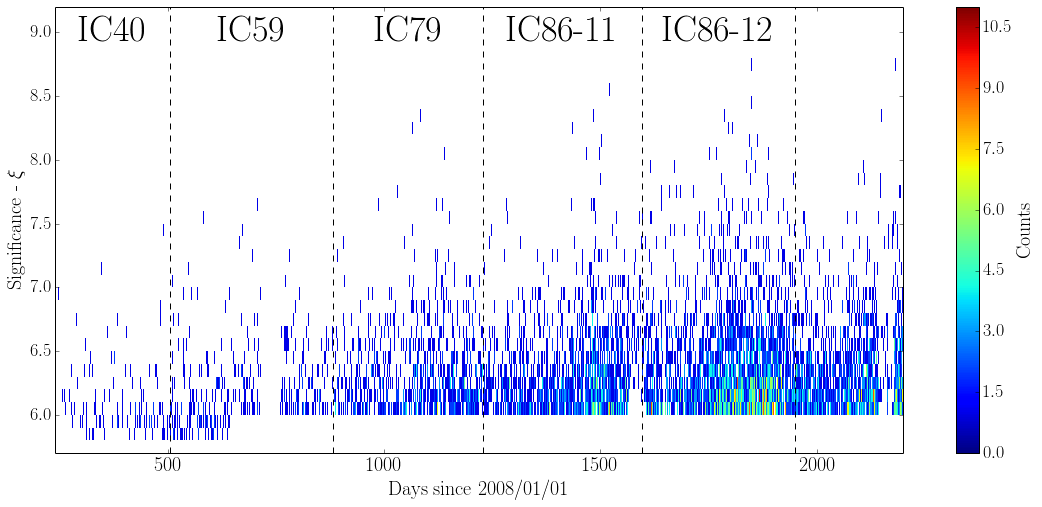
\includegraphics[width=1\textwidth]{./figures/IC40IC863AlertsSigmavsTwebsiteparser.png}
  \end{center}
  \caption{SNDAQ significances, $\xi$, over threshold (6) from IC40 to present. \label{fig:SNDAQtriggershisto}}   
\end{figure}

% \begin{figure}[h]
%   \begin{center}
%     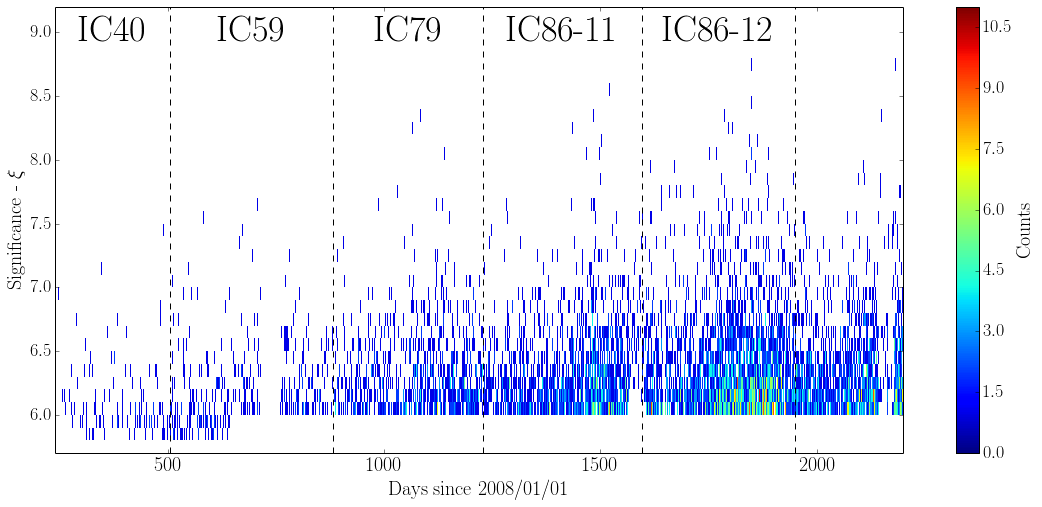
\includegraphics[width=1\textwidth]{./figures/IC40IC863AlertsSigmavsTwebsiteparser.png}
%   \end{center}
%   \caption{SNDAQ significances, $\xi$, over threshold (6) from IC40 to present. \label{fig:muratetriggersig}}   
% \end{figure

% \begin{figure}[h]
%   \begin{center}
%     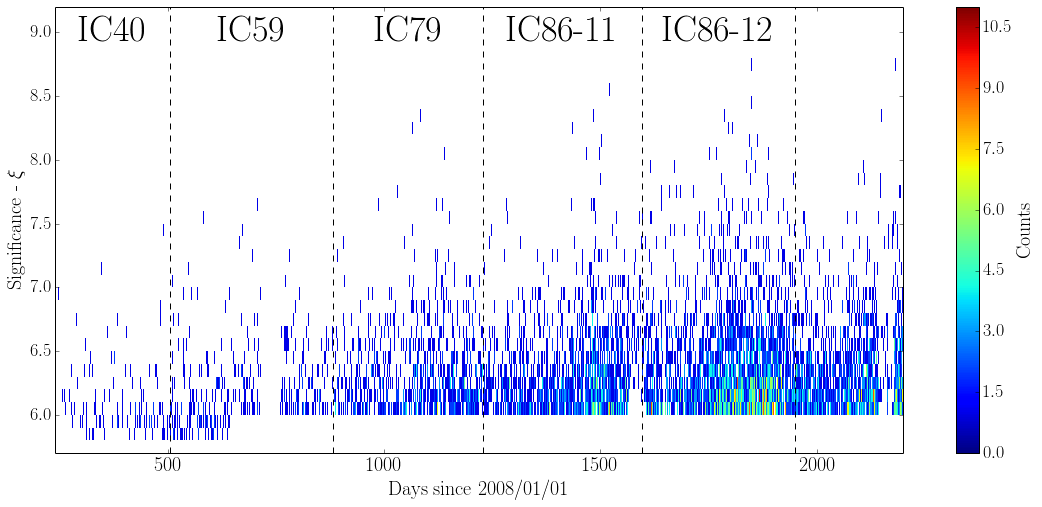
\includegraphics[width=1\textwidth]{./figures/IC40IC863AlertsSigmavsTwebsiteparser.png}
%   \end{center}
%   \caption{SNDAQ significances, $\xi$, over threshold (6) from IC40 to present. \label{fig:solarcycle}}   
% \end{figure}

In \cite{vbaumaster} the Data Storage Tape (DST) data was used determine the muon hit rate from the SMT8 trigger rate and the number of DOMs that were triggered, ``nchannel'' (nchan), of the triggers. This muon hit rate is shown to be correlated to the $\xi$ as determined by the the supernova online analysis. There was however no consideration for other triggers, such as the \emph{String Trigger} and the \emph{Volume Trigger}. These triggers could help identify large muon events that cause false supernova triggers more readily. For this reason, a study of the correlation of trigger rates for SMT8, SMT3, Volume Trigger, and String Trigger with supernova false trigger will be performed. For the supernova false triggers with $\xi > 6$, the trigger rate for all triggers of interest will be determined from the Super Data Storage Tape (sDST). The sDST data contains all individual triggers and time stamps thereof. The DST data only contains a bitmask that accounts for the the presence of a trigger, but not a count. This will help in account for possible overlapping triggers and give a better picture of the timing distribution. In order to ensure proper comparison of the data, the same rolling window as used in the SNDAQ online analysis is applied to the sDST data. The data is than split into the background and signal region and comparison of the trigger rates, nchannel distributions, and direction of events will be performed.

Investigating other triggers will remove some of the shortcomings of the analysis in \cite{vbaumaster}:

\begin{itemize}
  \item SMT8 rate of DST data does not reflect the real SMT8 rate
  \item SMT8 trigger does not consider any geometry information beyond the local coincidence (LC) condition
  \item Supernova scalers have a lower energy cutoff than SMT8, i.e. is SMT8 the best possible measure or is there a different trigger?
\end{itemize}

The DST does not contain all the trigger information, as overlapping triggers are compressed into a bitmask that only accounts for the the presence of a trigger, but not a count. SMT8 triggers can overlap because of their extended readout windows as required by the EventBuilder. The probability of overlap of two SMT8, assuming \unit[2100]{Hz} trigger rate for SMT8 and a \unit[10]{$\mu$s} readout overlap window, is $\approx$ 0.2\%. This should have an minuscule effect on the correlation method. When looking at all possible triggers the overlap between different triggers approaches 1. Additional other triggers, mainly the \emph{Volume Trigger}, have a much higher rate ($\approx \unit[3300]{Hz}$), which leads to a much higher possibility of overlap for these triggers. 

The SMT8 trigger does not consider the geometry of the events and the detector beyond the geometry requirement of the local coincidence (LC) condition. The geometry and time span of a muon event are completely different than that for a supernova event. Individual muon events would only illuminate certain areas of the detector for $\mathcal{O}$(\unit[1 - 10]{$\mu$s}), while the supernova event illuminates the entirety of the detector over the course of $\mathcal{O}$(\unit[1 - 10]{s}). Looking at triggers that do have stricter geometric constrains may help identifying muon events. Also the \emph{Volume Trigger}'s much higher rate may yield more information about lower energy muons that the supernova scalers are sensitive to, but not SMT8. 

In addition to the trigger rate aspect. The comparison of nchan distribution and the location of the ``center-of-gravity'', where most of the hits are clustered, of the events between the signal region and the background region will be performed. 


  % \item Sensitivity of SMT8 trigger to supernova signals was never established


\section{Ice Efficiency}

The optical properties of the ice in which IceCube is embedded are not uniform throughout the detector. One of the main assumptions that goes into the supernova onlien analysis a uniform illumination of the ice by the interaction of supernova neutrinos. The different optical properties however will cause the ice to not be illuminated uniformly, as some DOMs will have greater sensitivity than others because the light from the products of supernova neutrino interactions can travel more readily through the ice.

From studying the ice properties versus depth for MeV-scale positrons, one can establish an efficiency factor for the ice surrounding the DOM. To do this, an average of the effective volume of the DOMs outside the dust layer is calculated for an IceCube. The DOMs in the dust layer are excluded from the average because of the poor optical properties of the ice and the articifical decrease of the average effectice volume this would produce. The ratio between the average and the effective volume for the DOM is defined as the ice efficiency parameter. The effective volume of the DeepCore DOMs has to adjusted from the higher quantum efficiency as this effect is already taken into account separately, but still be able to compensate for their different location inside the detector. 

% \section{SNDAQ Changes}

The likelihood used in the SNDAQ online analysis relies on assumption that the noise rate on a per DOM level is Gaussian distributed, i.e. that the noise is purely Poissonic in nature. The per-DOM noise rate over long time scales however is known to be log-normal distributed

\begin{equation}
    f_{X}(x; \mu, \sigma) = \frac{1}{x \sigma \sqrt{2\pi}} \textrm{exp} \left\{ -\frac{1}{2} \left( \frac{ln(x) - \mu}{\sigma}  \right)^{2} \right\}
\end{equation}

\noindent where $\mu$ is the location parameter and $\sigma$ is the scale parameter. Over a short time scales as used in the SNDAQ analysis, i.e. \unit[11]{minutes}, the log-normal behavior can be approximated with a Gaussian 

\begin{equation}
    f_{X}(x; \mu, \sigma) = \frac{1}{\sigma \sqrt{2\pi}} \textrm{exp} \left\{ -\frac{1}{2} \left( \frac{x - \mu}{\sigma}  \right)^{2} \right\}
\end{equation}

\noindent where $\mu$ is the mean and $\sigma$ is the standard deviation or variance. 

Given Gaussian behavior of the DOM noise, we can measure a collective increase rate of the detector, $\Delta \mu$, employing the likelihood

\begin{equation}
    \mathcal{L}(\Delta \mu) = \prod_{i=1}^{N_{\textrm{DOM}}} \frac{1}{\sigma_{i} \sqrt{2\pi}} \textrm{exp} \left\{ -\frac{1}{2} \left( \frac{r_{i} - (\mu_{i } + \epsilon_{i}\Delta \mu)}{\sigma_{i}}  \right)^{2} \right\}
\end{equation}

\noindent where $r_{i}$ is the rate in the signal bin, $\mu_{i}$ and $\sigma_{i}$ is the average rate and error on the average rate estimated from the background region. From maximizing the log-likelihood we can obtain an analytical form of $\Delta \mu$:

\begin{equation}
  \Delta \mu = \sigma_{\Delta \mu} \sum_{i = 1}^{N_{\textrm{DOM}}} \frac{\epsilon_{i}}{\sigma_{i}} (r_{i} - \mu_{i})
\end{equation}

\noindent where 

\begin{equation}
  \sigma_{\Delta \mu} = \left( \sum_{i = 1}^{N_{\textrm{DOM}}} \frac{\epsilon_{i}^{2}}{\sigma_{i}^{2}} \right)^{-1}
\end{equation}

The assumption of purely Poissonic noise however appears to break down to do the non-Poissnic nature of the muon background on a per-DOM basis. A possible solution for this is the use a likelihood based on a log-normal distribution:

\begin{equation}
    \mathcal{L}(\Delta \mu) = \prod_{i=1}^{N_{\textrm{DOM}}} \frac{1}{\sigma_{i} r_{i} \sqrt{2\pi} } \textrm{exp} \left\{ -\frac{1}{2} \left( \frac{ln(r_{i}) - (\mu_{i} + \epsilon_{i}\Delta \mu)}{\sigma_{i}}  \right)^{2} \right\}
\end{equation}

\noindent where 

\begin{equation}
  \mu_{i} = ln\left( \frac{m^{2}}{\sqrt{ v + m^{2}}}\right)
\end{equation}

\noindent and

\begin{equation}
  \sigma_{i} = \sqrt{ ln(1 + \frac{v}{m^{2}}) }
\end{equation}

\noindent $m$ and $v$ are the mean and variance of the data, respectively. This changes $\Delta \mu$, such that

\begin{equation}
  \Delta \mu = \sigma_{\Delta \mu} \sum_{i = 1}^{N_{\textrm{DOM}}} \frac{\epsilon_{i}}{\sigma_{i}} (ln(r_{i}) - \mu_{i})
\end{equation}

\begin{thebibliography}{2}

\bibitem{vbaumaster} V. Baum, Verbesserung Der Supernova-Detektion Mit Dem IceCube-Neutrinoteleskop, Johannes Gutenberg-Universit\"{a}t Mainz, 2011.

\bibitem{mkrasbergtalk} M. Krasberg, Low-Level Commissioning, IceCube Collaboration Meeting Baton Rouge, 2006

\end{thebibliography}

\end{document}
